%! TEX root = ./thesis.tex
\chapter{Suchprobleme und die Hypothese $\hQ$ im Kontext des Pudlákschen Programms}\label{chap:pudlak}


In der Einleitung dieser Arbeit wurde bereits angedeutet, dass die Hypothese $\hQ$ von \citeauthor{fenner_inverting_2003} große Nähe und Verwandtschaft zu Hypothesen hat, die Suchprobleme im Allgemeinen und Beweissystemen im Speziellen betreffen. Damit ergeben sich Beziehungen zu Hypothesen aus dem Pudlákschen Programm, insbesondere $\neg\hSAT$ (also dass eine NP-vollständige Mengen mit $\P$-optimalem Beweissystem für diese Menge existiert).
In diesem Kapitel werden wir diese Beziehungen näher erarbeiten. Zur Erinnerung:

\begin{reptheorem}{Vermutung}{conj:q}[$\hQ$, \cite{fenner_inverting_2003}]
    Für jede totale NPTM $N$ (d.h. $L(N)=\Sigma^*$) existiert eine Funktion $g\in\FP$ sodass für alle $x$ das Bild $g(x)$ ein akzeptierender Rechenweg von $N(x)$ ist. 
\end{reptheorem}

Im Kapitel werden wir uns grob folgenden drei Desiderata widmen: 
erstens, nähern wir uns in Abschnitt~\ref{sec:karp-vs-levin} erneut der Frage zwischen Levin- und Karp-Vollständigkeit bzw. der Hypothese $\mathsf{KvL}$ aus vorigem Kapitel. Insbesondere analysieren wir die Beziehungen von $\mathsf{KvL}$ zu $\hQ$ und versuchen, $\mathsf{KvL}$ in das Pudláksche Programm einzuordnen.

Zweitens, in Abschnitt~\ref{sec:q-vs-search}, verallgemeinern wir Charakterisierungen $\hQ$, die sich insbesondere auf Suchprobleme und deren assoziierte Beweissysteme beziehen.
Insbesondere zeigen wir für eine große Klasse von vollständigen NP-Suchproblemen $R$ (nämlich jene die Levin-paddable sind) dass das zu $R$ assoziierte \emph{Standardbeweissystem} ($(x,y)$ mit $R(x,y)$ ist ein Beweis für $x$) $\P$-optimal ist, genau dann wenn $\hQ$. Damit wird die $\P$-Optimalität des entsprechenden Standardbeweissystems zu einer Invariante, die entweder für \emph{alle} Levin-paddable NP-Suchprobleme zutrifft, oder für \emph{keins}.

%erstens werden wir weitere Hypothesenzu Suchproblemen, welche sich im Verlauf dieser Arbeit ergeben, in das Pudláksche Programm einordnen, insbesondere $\hQ$ und $\mathsf{KvL}$ bzw. die Frage nach Levin- vs. Karp-Vollständigkeit.
%Im Speziellen ergänzen wir das Abbildung~\ref{fig:pudlak} der Beziehungen zwischen den Pudlákschen Hypothesen aus der Einleitung um weitere Hypothesen, und erreichen Abbildung~\ref{}. Die Beweise 

%Zweitens eine Verallgemeinerung der Charakterisierung $\hQ$, die sich insbesondere auf Suchprobleme und deren Beweissysteme bzw. „Zertifikatsschemata“ beziehen.

Drittens ergänzen wir im gesamten Verlauf dieses Kapitels das Pudláksche Programm um weitere Hypothesen ($\mathsf{KvL}, \hQ, \dots$), sodass Abbildung~\ref{fig:pudlak-small} der Beziehungen zwischen den Pudlákschen Hypothesen vergrößert wird. Damit erreichen wir den Stand, der in Abbildung~\ref{fig:figure-implications} dargestellt wird.
Damit einher wird abschließend ein Überblick über Orakel angegeben, welche Hypothesen des Pudlákschen Programms (ergänzt um $\hQ, \mathsf{KvL}, \dots$) trennen.


Für alle dieser drei Desiderata ist es zunächst notwendig, auf die Hypothese $\hQ$ einzugehen.
\textcite{fenner_inverting_2003} beobachten, dass das Invertieren von surjektiven ehrlichen FP-Funktionen eine erstaunlich robuste Aussage ist, die eine Vielzahl von äquivalenten „fundamentalen“ \parencite{fenner_inverting_2003} Charakterisierungen aus der Komplexitätstheorie zulässt, so zum Beispiel die effiziente Lösbarkeit von TFNP-Suchproblemen, oder das effiziente Ausrechnen akzeptierender Rechenwege einer totalen NPTM. Wir können jetzt schon festhalten, dass die aktuelle Forschung diese Hypothese als sehr stark einschätzt, und eher die negative Beantwortung (i.e. $\neg\hQ$) vermutet.


\begin{theorem}[Äquivalente Formulierungen der Hypothese $\hQ$; \cite{fenner_inverting_2003}]\label{thm:q-orig}
    Folgende Aussagen sind äquivalent:
    \begin{enumerate}
        \item Hypothese $\hQ$.
        \item $\mathrm{NPMV}_t\subseteqc \mathrm{FP}$.
        \item $\TFNP\subseteqc \mathrm{FP}$.
        \item $\P=\NP\cap\coNP$ und $\mathrm{NPMV}_t\subseteqc \mathrm{NPSV}_t$.
        \item Jede surjektive ehrlichen Funktion $f\in\FP$ ist $\P$-invertierbar.
        \item Für jede Menge $L\in \P$  und jede NPTM $N$ mit $L(N)=L$ existiert eine Funktion $h\in \FP$ mit 
            \[ x\in L \implies N(x) \text{ akz. mit Rechenweg $h(x)$}. \]
    \end{enumerate}
\end{theorem}

\textcite{fenner_inverting_2003} und \textcite{messner_simulation_2001} charakterisieren $\hQ$ noch durch zwei weitere Formen, diesmal über je eine Aussage über die Menge $\mathtt{SAT}$:

\begin{restatable}{theorem}{qfennermessner}\label{thm:q-fenner-messner}
    Folgende Aussagen sind äquivalent:
\begin{enumerate}[midpenalty=0,endpenalty=10000]
        \item Hypothese $\hQ$.
        \item \parencite{fenner_inverting_2003} Für jede NPTM $N$ mit $L(N)=\mathtt{SAT}$ existiert eine Funktion $h\in \FP$ sodass 
\[ N(\phi) \text{ akz. mit Rechenweg $w$} \implies \text{$h(w)$ ist eine erfüllende Belegung für $\phi$.} \]
        \item \parencite{messner_simulation_2001} Das Standardbeweissystem $\mathit{sat}$
            \[ \mathit{sat}(\phi, w) = \begin{cases} \phi & \text{wenn $w$ eine erfüllende Belegung für $\phi$ ist} \\ \bot & \text{sonst.} \end{cases}\]
            für $\mathtt{rSAT}$ ist $\P$-optimal.
    \end{enumerate}
    Dieser Satz relativiert nicht.
\end{restatable}

In anderen Worten sagt Aussage (2) aus, dass es modulo Umcodieren nur einen einzigen SAT-Solver gibt, und insbesondere alle SAT-Solver äquivalent zum trivialen Solver ist, welcher nur alle möglichen Belegungen ausprobiert.
Die Aussage (3) macht eine analoge Aussage über Beweissysteme: egal wie komplex ein Beweissystem $h$ für $\mathtt{SAT}$ ist, wir können immer einen $h$-Beweis für $\phi$ in eine erfüllende Belegung für $\phi$ (quasi ein trivialer Beweis für $\phi\in\mathtt{SAT}$) transformieren. Damit ist auch leicht zu sehen, dass $\hQ\Rightarrow \neg\hSAT$, zumindest im unrelativierten Fall.

In Abschnitt~\ref{sec:q-vs-search} werden wir sehen, dass sich die obigen Charakterisierungen auf weitere (aber möglicherweise nicht alle) vollständigen NP-Relationen generalisiert, womit insbesondere auch die beiden Charakterisierungen von \citeauthor{fenner_inverting_2003} und \citeauthor{messner_simulation_2001} zu einer \emph{relativierbaren} Variante verallgemeinert werden.
Mit dieser Verallgemeinerung ist es dann auch für uns möglich, $\hQ$ formal in das Pudláksche Programm (u.a. durch $\hQ\Rightarrow \neg\hSAT$) einzuordnen. Hierfür führen wir jetzt schon den Begriff eines Standardbeweissystems formal ein.

\begin{definition}[Standardbeweissystem einer NP-Relation]
    Sei $R$ eine NP-Relation. Wir definieren bezüglich $R$ das \emph{Standardbeweissystem} $\mathit{std}_R$ für $\Proj(R)$ wie folgt:
    \[ \mathit{std}_R(w) \defeq \begin{cases} x & \text{wenn $w=(x,y)$ und $(x,y)\in R$,}\\
    \bot & \text{sonst}.\end{cases} \qedhere \] 
\end{definition}
Damit ist, wie durch die Formulierung oben suggeriert, $\mathit{sat}=\mathit{std}_{\mathtt{rSAT}}$.
Bevor wir nun mit einer Diskussion zwischen Karp-Vollständigkeit und Levin-Vollständigkeit fortsetzen, schließen wir diesen Einstieg mit folgender einfachen Beobachtung ab:
\begin{observation}\label{obs:spps-honest}
    Für jede NP-Relation $R$ ist das Standardbeweissystem $\mathit{std}_R$ für $\Proj(R)$ ehrlich, optimal, und hat kurze Beweise.
\end{observation}
\begin{proof}
    Nachdem $R$ polynomiell längenbeschränkt ist, folgt sofort dass $\mathit{std}_R$ kurze Beweise hat. 
    Nach Beobachtung \ref{obs:super-ps-sind-opt} damit auch optimal.
    Insbesondere hat $\mathit{std}_R$ \emph{nur} polynomiell längere Beweise, also ist $\mathit{std}_R$ ehrlich.
\end{proof}
%\begin{proof}
    %Sei $q$ die Zertifikatsschranke von $R$, und sei $w=(x,y)$ gegeben sodass $\mathit{std}_R(x,y) = x$.
    %An dieser Stelle müssen wir auf die konkrete Codierung von Beweisen $w=(x,y)$ eingehen.
    %Wie in \ref{sec:notation} beschrieben, codieren wir Tupel in einer solchen Weise sodass
    %\[ |w| = |(x,y)| = 2(|x|+|y|+2) = 2|x|+ 2|y| + 4. \]
    %Da $(x,y)\in R$ gilt für $y$ auch $|y|\leq q(|x|)$.
    %Damit also
    %\[ |w| \leq 2|x|+ 2q(|x|) + 4 \leq q'(|x|) = q'(|\mathit{std}_R(w)|). \]
    %für ein geeignetes Polynom $q'$, wie gewünscht.
%\end{proof}

\begin{figure*}
    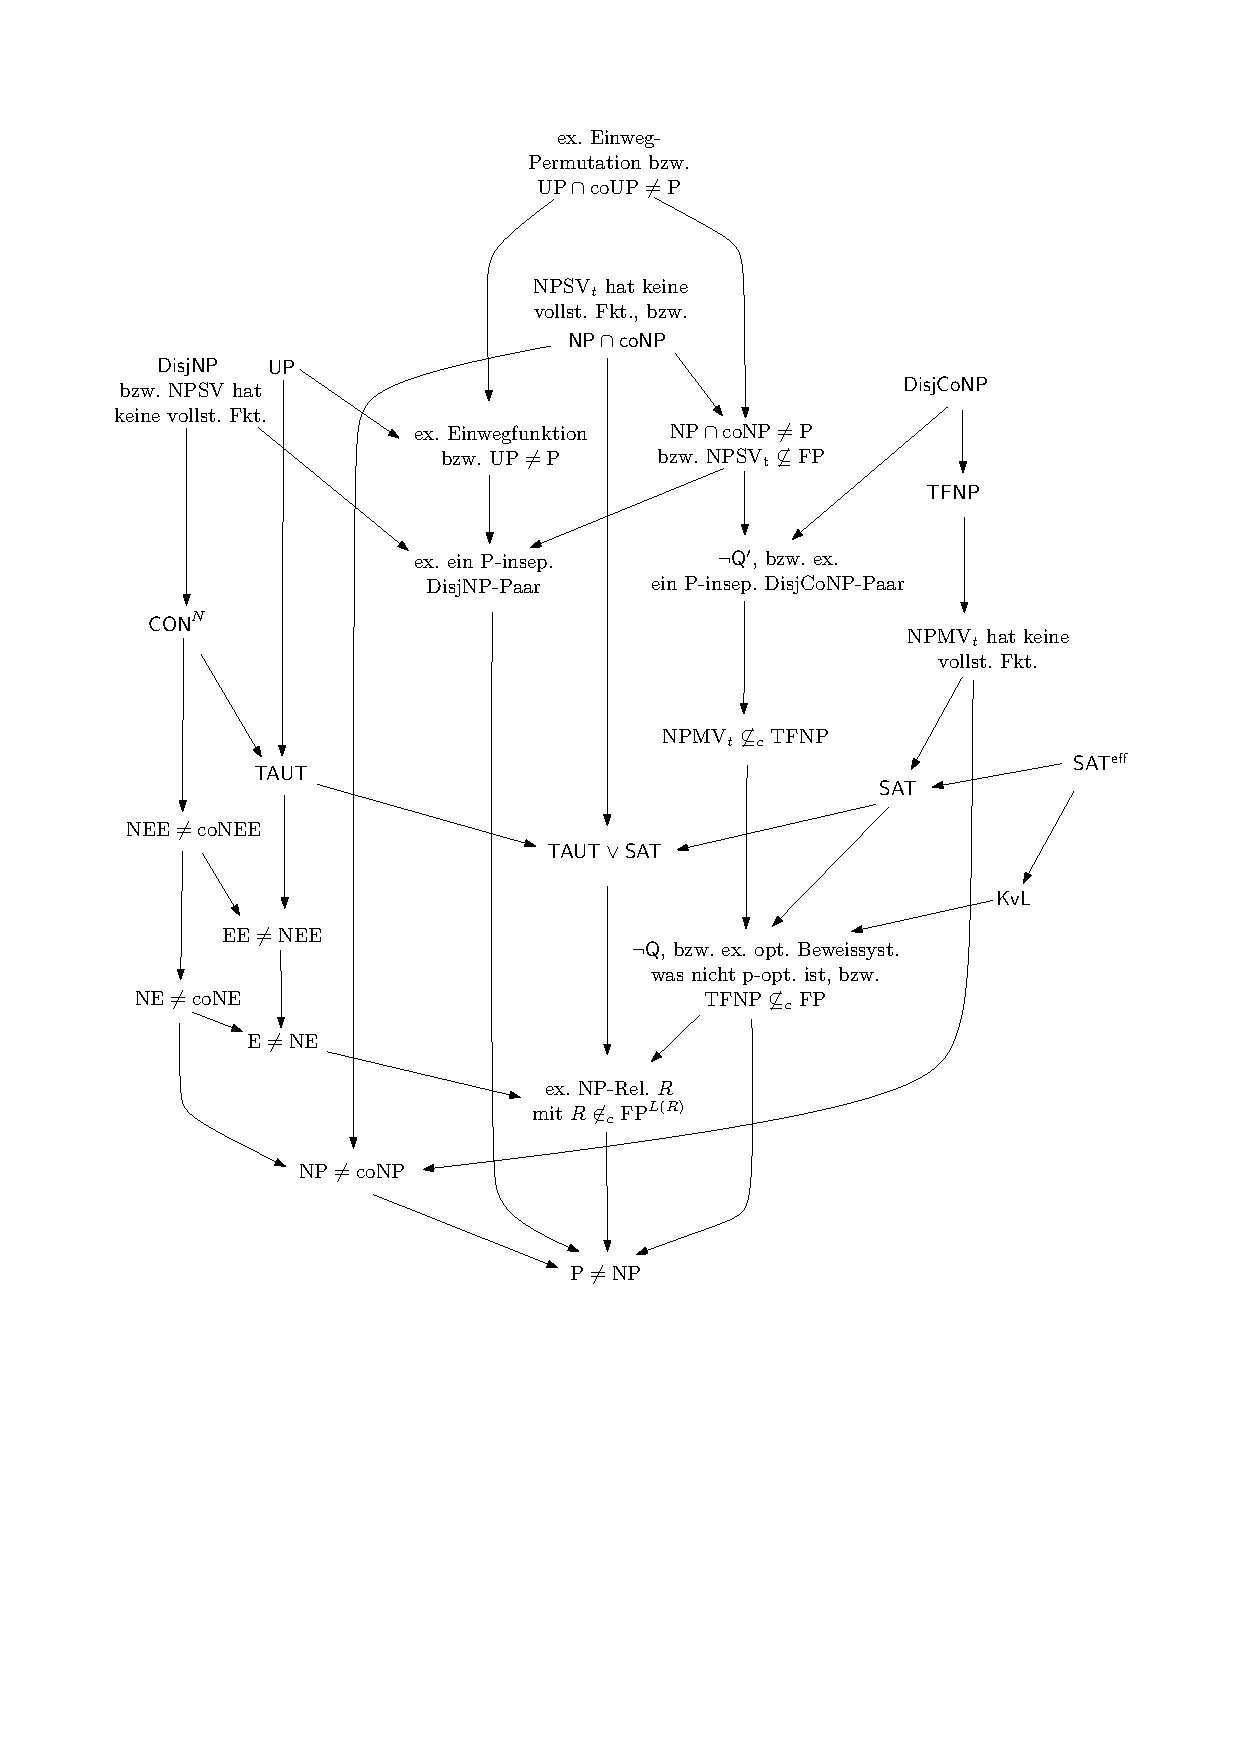
\includegraphics[page=1]{figures.pdf}
    \caption{Bekannte (relativierenden) Implikationen zwischen den betrachteten Hypothesen und weiteren Aussagen. Satz~\ref{thm:figure-implications} gibt Belegstellen für jede dieser Implikationen an.}\label{fig:figure-implications}
    \forcerectofloat
\end{figure*}

\section{Karp-Vollständigkeit vs. Levin-Vollständigkeit}\label{sec:karp-vs-levin}

Wir wiederholen hier erneut die zentrale offene Frage und Vermutung aus Abschnitt~\ref{sec:levin}:

\begin{reptheorem}{Frage}{question:kvl}
Wenn $\Proj(R)$ eine $\leqmp$-vollständige Menge für $\NP$ ist, ist dann auch $R$ eine $\leqlp$-vollständige NP-Relation für $\FNP$?
\end{reptheorem}

\begin{reptheorem}{Vermutung}{conj:kvl}[$\mathsf{KvL}$]
    Es existiert eine NP-Relation $R$ sodass $\Proj(R)$ $\leqmp$-vollständig für $\NP$ ist, aber $R$ ist nicht $\leqlp$-vollständig für $\FNP$.
\end{reptheorem}

Zunächst sei hier noch einmal hervorgehoben, dass eine Beantwortung der Frage~\ref{question:kvl} schwer ist. Zum einen haben wir bereits gesehen, dass ein Beweis $\mathsf{KvL}$ auch sofort $\P\neq\NP$ berweisen würde. Insbesondere ist ein relativierender Beweis von $\mathsf{KvL}$ ausgeschlossen, denn existiert ein Orakel, relativ zu diesem $\neg\mathsf{KvL}$ (z.B. ein PSPACE-vollständiges Orakel, welches $\NP$ auf $\P$ kollabiert).

Wir werden uns daher im Folgenden insbesondere auf Beziehungen zwischen Hypothesen und $\mathsf{KvL}$ konzentrieren.
In diesem Sinne möchte ich argumentieren, dass die obige Frage bzw. Vermutung eng mit der Hypothese $\hQ$ zusammenhängt.
Im Speziellen werden wir sehen, dass die Hypothese $\hQ$ so charakterisiert werden kann, dass sie einer Verstärkung der Vermutung $\neg\mathsf{KvL}$ entspricht.\footnote{\textcite{fenner_inverting_2003} gaben hierbei eine ähnliche Aussage an (Cor.~3: „$\hQ$ holds iff every Karp reduction from $A$ to $B$ can be extended to a Levin reduction“), es ist aber hervorzuheben, dass die Autoren von einem unüblichen Begriff von Levin-Reduktionen ausgehen, der sich von dem hier verwendeten unterscheidet. Dieser umfasst nicht eine „Rückwärts-Translation“ von Zertifikaten für $B$-Instanzen zu $A$-Instanzen, sondern eine „Vorwärts-Translation“ von Zertifikaten für $A$-Instanzen zu $B$-Instanzen.}

\begin{theorem}\label{thm:q-as-levin}
    Folgende Aussagen sind äquivalent:
    \begin{enumerate}
        \item Hypothese $\hQ$, bzw. $\TFNP\subseteqc\FP$. 
        \item Für jedes Paar von NP-Relationen $A, B$ gilt:
            \[ \Proj(A) \leqmp \Proj(B) \iff A \leqlp B. \]
    \end{enumerate}
\end{theorem}
\begin{proof}
    \begin{prooflist}
\item (1)$\implies$(2): Die Richtung von rechts nach links ist klar. Für die andere Richtung sei $\Proj(A) \leqmp \Proj(B)$ mit $A,B$ NP-Relationen. Sei $q$ hierbei das Polynom was die Zertifikatslänge in $A$ begrenzt.
    Wir wollen nun eine Levin-Reduktion von $A$ auf $B$ angeben. Sei $f\in \FP$ die Funktion, welche die Reduktion $\Proj(A) \leqmp \Proj(B)$ realisiert.

    Definiere folgende Relation $R$ mit
    \[ \fset{}R(w) = \begin{cases} \{ y\mid y\in\Sigma^{\leq q(|x|)}, (x,y)\in A \} & \text{falls $w=(x,y')$, $(f(x), y')\in B$} \\  \{\epsilon\} & \text{sonst}. \end{cases} \]
    Es ist leicht zu sehen, dass $R$ eine totale NP-Relation ist. Nach (1) existiert nun eine (totale) Verfeinerung $g\in \FP$ von $R$.

    Damit lässt die Levin-Reduktion von $A$ auf $B$ angeben: wähle $f$ als Reduktionsfunktion, und sei die Funktion $g$ von oben die Translationsfunktion. Dann gilt
    \begin{gather*}
        (f(x), y') \in B \implies (x, y')\in\Proj(R) \\
        \implies ((x, y'), g(x, y'))\in R\\
        \implies (x, g(x, y')) \in A \text{ nach Def. von $R$}
    \end{gather*}
    wie gewünscht. Wir haben $A\leqlp$ via $f, g$.
\item (2)$\implies$(1): Sei $A$ eine totale NP-Relation
    Definere nun die NP-Relation
    \[ B \defeq \{ (x, \epsilon) \mid x\in\Sigma^* \}. \]
    Es ist leicht zu sehen das $\Proj(A)=\Sigma^*=\Proj(B)$ und dass $\Proj(A)\leqmp\Proj(B)$ über die Identitätsfunktion.
    Nach Annahme (2) lässt sich nun diese Reduktion zu einer Levin-Reduktion $A\leqlp B$ verstärken, mit Reduktionsfunktion $f\in\FP$ und  Translationsfunktion $g\in\FP$.
    Für alle $x$ gilt nun $(f(x),\epsilon)\in B$ nach Definition,
    nach Levin-Reduktion also auch $(x, g(x, \epsilon))\in A$.
    Definieren wir nun $h(x)\defeq g(x,\epsilon)$, dann ist $(x, h(x))\in A$ für alle $x$, also $h\in\FP$ eine Verfeinerung von $A$, also $A\inc \FP$, wie gewünscht.
\end{prooflist}
\end{proof}

Beachte, dass in Aussage (2) die Implikation von rechts nach links ohnehin immer gilt. 
Damit lässt sich Aussage (2) auch so formulieren, dass jede Karp-Reduktion zu einer Levin-Reduktion verstärkt werden kann, indem zur Reduktionsfunktion $f$ eine geeignete Translationsfunktion $g$ hinzugefügt wird.
Mit dieser Charakterisierung folgt auch unmittelbar, dass $\hQ$ hinreichend für $\neg\mathsf{KvL}$ ist.


\begin{theorem}\label{thm:kvl-implies-q}
    $\mathsf{KvL} \implies \neg\hQ$.
\end{theorem}
\begin{proof}
    Wir zeigen die Kontraposition, und starten mit der Voraussetzung $\hQ$.
    Wir wollen nun $\neg\mathsf{KvL}$ zeigen. Sei hierfür $R$ eine beliebige NP-Relation sodass $\Proj(R)$ $\leqmp$-vollständig ist.
    Damit gilt also schon für alle weiteren NP-Relationen $A$, dass $\Proj(A)\leqmp\Proj(R)$.
    Nach Satz~\ref{thm:q} gilt also auch die Aussage \ref{thm:q}(6), und damit $A\leqlp R$. Also ist $R$ auch $\leqlp$-vollständig, wie gewünscht und wir haben $\neg\mathsf{KvL}$ gezeigt.
\end{proof}

Was sind natürlich notwendige Bedingungen für die Hypothese $\mathsf{KvL}$? Diese Frage erscheint tatsächlich wesentlich schwieriger als gedacht. Insbesondere scheint es unklar, ob aus irgend einer von Pudláks Hypothesen die Aussage $\mathsf{KvL}$ folgt.

Besonders interessant erscheint aber die Beziehung zur Hypothese $\neg\hQ$, also genau die Umkehrung von Satz~\ref{thm:kvl-implies-q}.
Zumindest in der obigen Charakterisierung durch Satz \ref{thm:q-as-levin} scheint $\neg\hQ$ schwächer, denn die Negation von Satz \ref{thm:q-as-levin}(2) würde aussagen, dass ein \emph{beliebiges} Paar $A,B$ von NP-Relationen existiert mit $\Proj(A)\leqmp \Proj(B)$, aber $A \not\leq_\mathrm L^\mathrm p B$. Weder $A$ noch $B$ müssen eine $\leqmp$-vollständige Projektion haben, was $\mathsf{KvL}$ ja verlangt.

%, ist ja die Aussage (2) vom Satz~\ref{thm:q-as-levin} \emph{fast} in der Form „Karp-Vollständigkeit = Levin-Vollständigkeit“ ist.
Stattdessen scheint die Charakterisierung von $\neg\hQ$ durch \citeauthor{fenner_inverting_2003} in Satz~\ref{thm:q-fenner-messner}(2) dienlicher:
Betrachten wir hierbei exemplarisch den Fall Relationen für $\mathtt{SAT}$. Ich vermute, dass $\neg\hQ\Rightarrow \mathsf{KvL}$; um das zu plausibilisieren möchte ich zeigen, dass $\neg\hQ\land\neg\mathsf{KvL}$ unwahrscheinlich ist.

Starten wir mit $\neg\hQ$, dann gilt mit Satz~\ref{thm:q-fenner-messner} für alle Funktionen $h\in\FP$
\begin{equation} N(\psi) \text{ akz. mit Rechenweg $w$} \rlap{\hspace*{2pt}\raisebox{2.3pt}{$\quad\not$}}\implies  (\psi, h(\psi, w))\in\mathtt{rSAT}.\label{eq:weak-irreducibility} \end{equation}
In anderen Worten: es existiert zwar eine NPTM $N$ welche $\mathtt{SAT}$ entscheidet, aber aus den akzeptierenden Rechenwegen $w$ von $N(x)$ auf $x\in \mathtt{SAT}$ kann nicht effizient eine akzeptierende Belegung für $x$ abgeleitet werden.

Wir können $N$ äquivalent als NP-Relation $R_N$ repräsentieren, mit $(\phi, w) \in R_N$ genau dann wenn $N(x)$ mit Rechenweg $w$ akzeptiert.
Damit kann Gleichung~\ref{eq:weak-irreducibility} so verstanden werden, dass $\mathtt{rSAT} \not\leqlp R_N$ \emph{falls die Reduktionsfunktion $f$ die Identitätsfunktion ist}.

Unter der Annahme $\neg\mathsf{KvL}$ existiert nun eine Levin-Reduktion $\mathtt{rSAT}\leqlp R_N$ mit Reduktions- bzw. Translationsfunktion $f,g$. Das ist zunächst kein Widerspruch, denn es könnte ja $f\neq\mathrm{id}$.
%
%An dieser Stelle muss erneut hervorgehoben werden, dass im Allgemeinen $\mathtt{rSAT} \leqlp R_N$ mit Funktionen $f,g$ gelten kann, notwendig hierfür ist aber dass $f\neq\mathrm{id}$.
%
Gleichzeitig wäre die Existenz einer solchen Reduktion überraschend. Wir hätten nach Definition
\begin{equation}\label{eq:effective-simulation} N(f(\phi)) \text{ akz. mit Rechenweg $w$} \implies \phi \text{ wird von Belegung $g(\phi, w)$ erfüllt}. \end{equation}
Einerseits ist es also nicht möglich, aus dem Rechenweg $w$ effizient eine akzeptierende Belegung für $f(\phi)$ zu bestimmen, obwohl $w$ bezeugt dass $f(\phi)$ erfüllbar ist. (Ersetze in \eqref{eq:weak-irreducibility} $\psi$ mit $f(\phi)$.)
Andererseits reicht der „Beweis“ $w$ aber aus, um (zusammen mit der Information $\phi$) effizient wieder eine erfüllende Belegung für $\phi$ zu berechnen. 
Das \emph{plausibilisiert} zwar einen Widerspruch, bzw. dass $\neg\hQ\land\neg\mathsf{KvL}$ wahrscheinlich falsch ist, ist aber natürlich kein solcher. Die Umkehrung von Satz~\ref{thm:kvl-implies-q} bleibt offen.

Dennoch vermute ich, dass solche Funktionen $f,g$ nicht jeweils für alle NPTM $N$ mit $L(N)=\mathtt{SAT}$ existieren können.
Tatsächlich können wir die eben formulierte Vermutung auch in der Theorie der Beweissystemen formulieren: hierfür können wir die beiden Aussagen aus Gleichung~\ref{eq:effective-simulation} je als Aussagen über „Beweissysteme“ verstehen. Links ist der Rechenweg $w$ der „Beweis“ für $f(\phi)\in \mathtt{SAT}$ über den Verifikator $N$, und rechts ist $g(\phi, w)$ die erfüllende Belegung für $\phi$, also ein $\mathit{sat}$-Beweis für $\phi\in\mathtt{SAT}$.

Um diese Idee nun zu formalisieren, definieren wir zunächst eine abgeschwächte Variante der $\P$-Simulation.
\begin{definition}
    Seien $h,h'$ Beweissysteme für $L$. Das Beweissystem $h$ \emph{$\P$-simuliert effektiv} $h'$ falls Funktionen $f,g\in\FP$ existieren sodass
    \begin{enumerate}
        \item $x\in L \iff f(x)\in L$,
        \item $ h'(w)=f(x) \implies h(g(x, w)) = x. $
    \end{enumerate}
    Wir schreiben in diesem Fall auch $h'\leq^\mathrm p_\mathrm{eff} h$. %\marginnote{\note{Nicht vergessen: es ist offenbar unklar, wie das Symbol $\leq$ bzgl. Simulation gebraucht wird. Dose/Glaßer würden in der Def. das Ordnungszeichen spiegeln, Krajíček/Pudlák dagegen genau so wie hier, Krajíček im Sammelband dagegen wieder gespiegelt.}}
\end{definition}
In anderen Worten, falls $h'\leq^p_\mathrm{eff} h$, dann kann $h$ zwar nicht \emph{jeden} $h'$-Beweis $w$ für $x\in L$ in einen $h$-Beweis für (das gleiche) $x$ effizient umrechnen, es kann aber zumindest alle \emph{relevanten} $h'$-Beweise effizient umrechnen, nämlich für jedes $x\in L$ die $h'$-Beweise für $f(x)$ in $h$-Beweise für $x$.
Anstelle „$h$ $\P$-simuliert effektv $h'$“ ließe sich äquivalent auch $h^{-1}\leqlp h'^{-1}$ schreiben. Beachte, dass die Relation $h^{-1}$ nur Lösungen mit ihren Beweisen reliert.
Klar ist: $\P$-Simulation impliziert effektive $\P$-Simulation impliziert Simulation unter Beweissystemen.

Die obige Intuition lässt sich also folgendermaßen formulieren: ich vermute, zumindest unter der Annahme $\neg\hQ$, dass das Standardbeweissystem $\mathit{sat}$ nicht jedes Beweissystem effektiv $\P$-simulieren kann, insbesondere nicht jenes was von der oben genannten NPTM $N$ induziert wird.
Wir können diese Vermutung auch allgemeiner ohne Bezugnahme auf $\mathtt{SAT}$ bzw. $\mathit{sat}$ formulieren:

\begin{conjecture}[$\mathsf{KvL}$ formuliert unter Beweissystemen]\label{conj:kvl-ps}
    Es existiert eine NP-Relation $Q$ mit $\leqmp$-vollständigem $\Proj(Q)$, wobei $\mathit{std}_Q$ nicht alle anderen optimalen Beweissysteme für $\Proj(Q)$ effektiv $\P$-simulieren kann.

    %In anderen Worten, es existiert ein optimales Beweissystem $h$ für $\Proj(R)$ sodass $h\not\leq^\mathrm p_\mathrm{eff}  \mathit{std}_R$.
    %Das Standardbeweissystem $\mathit{sat}$ für $\mathtt{SAT}$ kann nicht alle anderen optimalen Beweissysteme für $\mathtt{SAT}$ effektiv p-simulieren.

    %In anderen Worten, es existiert optimales Beweissystem $h$ sodass $h\not\leq^\mathrm p_\mathrm{eff} \mathit{std}$.
\end{conjecture}
%Beachte, dass in der obigen Formulierung $\mathit{std}_R$ \emph{nicht} „effektiv p-optimal“ ist in dem Sinn, dass \emph{jedes} Beweissystem effektiv p-simuliert werden kann, sondern eben nur die optimalen Beweissysteme bzw. genau jene mit kurzen Beweisen.
Dass die Formulierung der Vermutungen \ref{conj:kvl} und \ref{conj:kvl-ps} äquivalent sind, zeigt folgende Beobachtung:
\begin{observation}\label{obs:kvl-equiv}
    %Sei $R$ eine NP-Relation mit $\leqmp$-optimalem $\Proj(R)$.
    %Sei $L$ eine $\leqmp$-vollständige Menge für $\NP$.
    Folgende Aussagen sind äquivalent:
    \begin{enumerate}
        \item Für jede NP-Relation $R$ mit $\leqmp$-vollständigem $\Proj(R)$ ist $R$ $\leqlp$-vollständig. (Das ist die Aussage $\neg\mathsf{KvL}$.)
        \item Für jede NP-Relation $Q$ mit $\leqmp$-vollständigem $\Proj(Q)$ kann $\mathit{std}_Q$ jedes optimale Beweissystem $h$ für $\Proj(Q)$ effektiv $\P$-simulieren. (Das ist die Negation von der Vermutung~\ref{conj:kvl-ps}.)
        %\item Ist $\Proj(R)=L$, dann ist auch $R$ $\leqlp$-vollständig.
        %\item Ist $\Proj(R)=L$, dann gilt für alle optimalen Beweissysteme $h$ für $L$ auch $h\leq^\mathrm p_\mathrm{eff} \mathit{std}_R$.
    \end{enumerate}
\end{observation}
\begin{proof}
    \begin{prooflist}
    \item (1)$\Rightarrow$(2): 
        Sei $R$ eine NP-Relation mit $\leqmp$-vollständigem $\Proj(R)$.
    Wir zeigen, dass $\mathit{std}_{R}$ jedes andere optimale Beweissystem $h$ effektiv $\P$-simulieren kann.
    Nachdem $h$ optimal ist, hat es auch kurze Beweise (Beob.~\ref{obs:ps-for-np-optimal}): für jedes $x\in\Proj(R)$ existiert ein $h$-Beweis $w$ mit $|w|\leq q(|x|)$ für geeignetes Polynom $q$.  Definiere
    \[ R_h \defeq \{ (x, w) \mid |w|\leq q(|x|), h(w) = x\}. \]
    Diese Relation ist offenbar eine NP-Relation und $\Proj(R_h) = \Proj(R)$ und damit ist $\Proj(R_h)$ auch $\leqmp$-vollständig. 

    Nach Voraussetzung (1) ist also  $R_h$ auch $\leqlp$-vollständig.
    Insbesondere gilt also  auch $R \leqlp R_h$. Damit existieren also Funktionen $f,g\in\FP$ sodass
    $x\in \Proj(R) \leftrightarrow f(x)\in\Proj(R)$ und
    \[ (f(x), w) \in R_h \implies (x, g(x, w))\in R. \]
    Nach Definition gilt also 
    \[ h(w)=f(x) \implies \mathit{std}_R(g(x, w)) = x, \]
    und damit ist $h\leq^\mathrm p_\mathrm{eff} \mathit{std}_R$.

\item (2)$\Rightarrow$(1): 
    Sei $R$ eine NP-Relation wobei $\Proj(R)$ $\leqmp$-vollständig ist. Wir zeigen nun, dass $R$ auch $\leqlp$-vollständig ist.
    Sei hierfür $Q$ eine beliebige NP-Relation; wir wollen $Q\leqlp R$ zeigen.

    Aus der $\leqmp$-Vollständigkeit folgt unmittelbar die Existenz einer Reduktionsfunktion $f$ mit 
    \[ x\in \Proj(Q) \iff f(x) \in \Proj(R). \]
    Definiere
    \[ h(w) \defeq \begin{cases} x & \text{falls $w=(x,y)$ und $(f(x),y)\in R$} \\ \bot & \text{sonst.} \end{cases} \]
    Wir zeigen, dass $h$ ein Beweissystem für $\Proj(Q)$ ist. Es ist offenbar dass $h\in\FP$. Die Funktion $h$ ist korrekt: wenn $h(x,y)=x$ dann ist $f(x)\in\Proj(R)$ und nach Eigenschaft von $f$ auch $x\in\Proj(Q)$.
    Die Funktion $h$ ist vollständig: Sei $x\in\Proj(Q)$. Dann ist schon $f(x)\in\Proj(R)$ und es gibt ein $y$ mit $(f(x),y)\in R$. Also ist $(x,y)$ ein $h$-Beweis für $x$.

    Außerdem ist klar, dass $h$ kurze Beweise hat, damit ist $h$ auch optimal (Beob.~\ref{obs:ps-for-np-optimal}). % ist.\todo{warum?}
    Damit gilt nach (2) nun, dass $h\leq^\mathrm p_\mathrm{eff} \mathit{std}_Q$. Also existieren Funktionen $f',g'\in\FP$ sodass
    \[ x\in \Proj(Q)\iff f'(x)\in\Proj(Q),\quad h(w)=f'(x) \implies \mathit{std}_Q(g'(x,w))=x. \]%\implies (x,g(x,w))\in Q. \]
    Das reicht aus, $Q\leqlp R$ zu zeigen: wähle $f''(x)\defeq f(f'(x))$ als Reduktionsfunktion, dann gilt
    \begin{gather*}
        (f''(x), y)\in R \implies (f(f'(x)), y)\in R \implies h(\underbrace{f'(x),y}_{w})=f'(x) \\
    \implies \mathit{std}_Q(g'(x,w))=x \implies (x,g'(x,w))\in Q. \end{gather*}
    Die Translationsfunktion $g''$, welche $(x,y)$ zu $g'(x,w)$ übersetzt, lässt sich leicht angeben.
\end{prooflist}
\end{proof}

Mit der Definition der effektiven $\P$-Simulation und der eben bewiesenen äquivalenten Formulierung der Karp-vs-Levin-Vermutung lässt sich nun zumindest die Hypothese $\hSAT$ so verstärken, dass diese hinreichend für $\mathsf{KvL}$ ist.


\begin{conjecture}[$\mathsf{SAT^{eff}}$]
    Keine $\leqmp$-vollständige Menge $L\in\NP$ hat ein optimales Beweissystem $h$, welches alle anderen optimalen Beweissysteme für $L$ effektiv $\P$-simulieren kann. 
    %Es existiert eine Menge $L\in\NP$, und kein optimales Beweissystem für $L$ kann kann alle anderen optimalen Beweissysteme für $L$ effektiv p-simulieren.
    %In anderen Worten, für jedes optimales Beweissystem $h$ für $L$ existiert ein  optimales Beweissysteme $h'$ für $L$ sodass $h'\not\leq^\mathrm p_\mathrm{eff} h$.
\end{conjecture}

%Ähnlich wie bei $\hSAT$ können wir $\mathsf{SAT^{eff}}$ als „existenziell“ charakterisieren.
%\begin{lemma}
%    Folgende Aussagen sind äquivalent:
%    \begin{enumerate}
%        \item Es existiert eine $\leqmp$-vollständige Menge $A$ für $\NP$ sowie ein optimales Beweissystem $h$ für $A$, sodass $h$ jedes andere optimale Beweissystem für $A$ effektiv p-simulieren kann. (Das ist die Aussage $\neg\mathsf{SAT^{eff}}$.)
%        \item Für jede Menge $B\in\NP$ existiert ein optimales Beweissystem $g$ für $B$, welches jedes andere optimale Beweissystem für $B$ effektiv p-simulieren kann.
%    \end{enumerate}
%\end{lemma}
%\begin{proof}
%\begin{prooflist}[label={}]
%\item (2)$\Rightarrow$(1): Klar.
%
%\item (1)$\Rightarrow$(2): 
%\end{prooflist}
%\end{proof}

Wir sehen nun, dass $\mathsf{SAT^{eff}}$ eine Verstärkung von sowohl $\hSAT$ als auch $\mathsf{KvL}$ ist:
\begin{theorem}\label{thm:sateff-generalizes-sat}
    \begin{enumerate}
        \item $\mathsf{SAT^{eff}}\implies \hSAT$
        \item $\mathsf{SAT^{eff}}\implies \mathsf{KvL}$
    \end{enumerate}
\end{theorem}
\begin{proof}
\begin{prooflist}
\item Zu (1): Klar aus Kontraposition. Wenn $\neg\hSAT$, dann existiert für eine $\leqmp$-vollständige Menge $L\in\NP$ ein $\P$-optimales Beweissystem $h$ für $L$ existiert, dann kann dieses (optimale) $h$ auch alle anderen Beweissysteme $\P$-simulieren, und damit insbesondere auch alle optimalen Beweissysteme $h'$ effektiv $\P$-simulieren.

\item Zu (2): Wieder klar aus Kontraposition. Unter $\neg\mathsf{KvL}$ folgt mit der Formulierung aus Vermutung~\ref{conj:kvl-ps} dass für jede NP-Relation $Q$, $\Proj(Q)$ vollständig, das (optimale) Standardbeweissystem $\mathit{std}_Q$ alle optimalen Beweissysteme für $\Proj(Q)$ effektiv $\P$-simulieren kann. Das gilt dann insbesondere auch für die $\leqlp$-vollständige NP-Relation $\mathtt{rKAN}$, also hat die $\leqmp$-vollständige Menge $\mathtt{KAN}$ \emph{ein} Beweissystem, welches alle optimalen Beweissysteme effektiv $\P$-simulieren kann.
\end{prooflist}
\end{proof}

Wir haben also je eine notwendige ($\neg\hQ$) und eine hinreichende Hypothese ($\mathsf{SAT^{eff}}$) für $\mathsf{KvL}$. 
Nichtsdestotrotz bleiben noch viele Fragen offen, die wir hier aus Platzgründen nicht weiter verfolgen werden. 
Zum einen zur Charakterisierung von $\mathsf{KvL}$:
Wir konnten zwar $\mathsf{KvL}$ als Aussage über Beweissysteme formulieren, aber sind auch andere äquivalente Aussagen möglich, z.B. ähnlich wie bei $\hQ$?

Zum anderen die Beziehungen zwischen $\mathsf{KvL}$ und anderen Hypothesen bzw. Annahmen.
Gibt es natürliche (z.B. kryptographische) Annahmen die hinreichend für $\mathsf{KvL}$ sind? Wie ist die Beziehung zu den anderen Pudlákschen Hypothesen? Wie verhält sich insbesondere $\hSAT$ zu $\mathsf{SAT^{eff}}$? 
Diese Fragen werden wir zum Teil in Kapitel~\ref{chap:orakel} klären; dort wird ein Orakel konstruiert, welches zeigt, dass selbst unter der Annahme von $\hDisjNP$ und $\hUP$ es nicht möglich ist, mit relativierenden Beweismethoden auf $\mathsf{KvL}$ zu schließen.
Wir kommen hierauf am Ende dieses Kapitels noch einmal zurück.

%Kann in Beobachtung~\ref{obs:kvl-equiv}(2) so verstärkt werden, dass $\mathit{std}_Q$ jedes (nicht nur die optimalen) Beweissystem effektiv p-simulieren kann, also gewissermaßen $\mathit{std}_Q$ „effektiv p-optimal“ ist?

Insgesamt ist durch die vorherigen Überlegungen aber ein erster Schritt getan, die Beziehung zwischen Levin- und Many-one-Vollständigkeit über die Vermutung $\mathsf{KvL}$ im Kontext des Pudlákschen Programms einzuordnen.
Weitere Forschung in diese Richtung erscheint vielversprechend.

\section{Hypothese $\hQ$ und Suchprobleme}\label{sec:q-vs-search}

Wie im Einstieg des Kapitels angesprochen, geben \textcite{fenner_inverting_2003} bzw. \textcite{messner_simulation_2001} äquivalente Charakterisierungen der Hypothese $\hQ$ an, welche sich im Wesentlichen auf auf der $\leqlp$-Vollständigkeit von $\mathtt{rSAT}$ aufbauen (Satz~\ref{thm:q-fenner-messner}).
Wir wiederholen hier noch einmal die Aussage, aber mit einer etwas abstrakteren Notation.
Ganz ähnlich wie NP-Relationen ein Standardbeweissystem induzieren, können wir auch das Standardbeweissystem bezüglich einer NPTM definieren:
\begin{definition}[Standardbeweissystem von NPTM]
    Sei $N$ eine NTM. Wir definieren bezüglich $N$ das das \emph{Standardbeweissystem} $\mathit{std}_N$ für $L(N)$ wie folgt:
    \[ \mathit{std}_N(w) \defeq \begin{cases} x & \text{wenn $w=(x,\alpha)$ und $N(x)$ akzeptiert auf RW $\alpha$,}\\
    \bot & \text{sonst}.\end{cases} \qedhere \] 
\end{definition}
Ähnlich wie bei Standardbeweissysteme für NP-Relationen ist $\mathit{std}_N$ für jede nichtdeterministische \emph{Polynomialzeit}-TM $N$ ehrlich, optimal, und hat kurze Beweise.
\begin{reptheorem}{Satz}{thm:q-fenner-messner}
    Folgende Aussagen sind äquivalent:
    \begin{enumerate}
        \item Hypothese $\hQ$.
        \item Für jede NPTM $N$ mit $L(N)=\mathtt{SAT}$ gilt $\mathit{std}_N\leqmp \mathit{sat}$. Es existiert also eine Funktion $h\in \FP$ sodass 
            \[ N(\phi) \text{ akz. mit Rechenweg $w$} \implies \text{$h(w)$ ist erfüllende Belegung für $\phi$}. \]
        \item Das Standardbeweissystem $\mathit{sat}$ für $\mathtt{rSAT}$ ist $\P$-optimal.
    \end{enumerate}
    Dieser Satz relativiert nicht.
\end{reptheorem}

%\begin{itemize}
    %\item Für jede NPTM $N$ mit $L(N)=\mathtt{SAT}$ existiert eine Funktion $h\in \FP$ sodass 
    %\[ N(\phi) \text{ akz. mit Rechenweg $w$} \implies \mathit{std}_{\mathtt{rSAT}}(\phi, h(w)), \]
    %i.e. $h(w)$ ist eine erfüllende Belegung für $\phi$.
    %\item Das Standardbeweissystem $\mathit{std}_{\mathtt{rSAT}}$ ist p-optimal.
%\end{itemize}
Diese beiden Charakterisierungen wollen wir im Folgenden verallgemeinern und auf beliebige $\leqlp$-vollständige NP-Relationen $R$ übertragen. 
Hieraus ergibt sich schon unmittelbar der technische Beitrag, dass dann diese Charakterisierungen auch in einer relativierten Umgebung angewendet werden können, um z.B. ein geeignetes Orakel zu konstruieren, was $\hQ$ von anderen Hypothesen trennt.

Zweitens ergibt sich aus der Verallgemeinerung das überraschende Ergebnis, dass $\leqlp$-Vollständigkeit allein zur Generalisierung nicht ausreicht. In den originalen Beweisen von \citeauthor{fenner_inverting_2003} und \citeauthor{messner_simulation_2001} wurden stillschweigend zusätzliche Eigenschaften von $\mathtt{rSAT}$ mitgedacht und ausgenutzt. Die folgende Generalisierung deckt diese Eigenschaften auf, und plausibilisiert dass diese womöglich nicht von allen $\leqlp$-vollständigen NP-Relationen geteilt werden.

Eine dieser stärkeren Eigenschaften von $\mathtt{rSAT}$, welche \citeauthor{fenner_inverting_2003} in ihren Beweisen gebrauchten, ist die $\leq_\mathrm{1,i}^\mathrm p$-Vollständigkeit von $\mathtt{rSAT}$. Wir schwächen im Folgenden diese Voraussetzunt ab, und verlangen nur, dass eine NP-Relation unter ehrlichen Reduktionen vollständig ist. Dies gilt insbesondere für $\mathtt{rSAT}$.
Für welche $\leqlp$-vollständigen NP-Relationen das noch zutrifft, werden wir unten betrachten.

Mit dieser ehrlichen Levin-Vollständigkeit lässt sich nun die Charakterisierung von \citeauthor[Thm.~2]{fenner_inverting_2003} generalisieren:
\begin{lemma}\label{lemma:q-generalized}
    Sei $R$ eine $\leqlp$-vollständige NP-Relation, mit der zusätzlichen Eigenschaft dass für die jeweilige entsprechende Problem-Reduktionsfunktion $f\colon Q\to R$ für $Q\leqlp R$ immer gilt, dass $f$ ehrlich ist.
Folgende Aussagen sind äquivalent:
\begin{enumerate}
    \item Aussage $\hQ$.
    \item Für alle NPTM $N$ mit $L(N)=\Proj(R)$ lassen sich akzeptierende Rechenwege von $N$ in Zertifikate umrechnen: es gilt $\mathit{std}_N\leqmp \mathit{std}_R$, bzw. existiert eine Funktion $h\in\mathrm{FP}$ sodass
        \[ N(x) \text{ akz. mit Rechenweg $\alpha$} \implies (x,h(x,\alpha))\in R. \]
\end{enumerate}
\end{lemma}
\begin{proof}
\begin{prooflist}
\item (1)$\Rightarrow$(2): 
    Nachdem $\hQ$ gilt, gilt auch $\TFNP\subseteqc\FP$ nach Beobachtung~\ref{obs:tfnp-q}.
    Sei nun $R$ eine beliebige NP-Relation mit Zertifikatsschranke $q$, und
    sei $N$ eine beliebige NPTM mit $L(N)=\Proj(R)$. 
    Definiere nun folgende Relation $Q$ mittels:
    \[ \fset{}Q(x, \alpha) \defeq  \begin{cases} \{ y\mid y\in\Sigma^{\leq q(|x|)}, (x,y)\in R \} & \text{falls $N(x)$ auf RW $\alpha$ akzeptiert,} \\\{\epsilon\} & \text{sonst.} \end{cases}\]
    Es ist leicht zu sehen, dass $Q$ eine totale NP-Relation ist. Insbesondere im ersten Fall gilt $x\in L(N)=\Proj(R)$, also existiert auch mindestens ein $y\in\fset{}R(x)$.

    Nach Annahme gilt also $Q\inc\FP$, sei also $h\in\FP$ eine Verfeinerung von $Q$.
    Nun gilt
    \begin{gather*}
        \mathit{std}_N(x,\alpha)=x\\
        \implies N(x) \text{ akz. mit Rechenweg $\alpha$}\\
        \implies \fset{}Q(x,\alpha) = \fset{}R(x)\\
        \implies h(x,\alpha) \in \fset{}R(x) \implies (x, h(x,\alpha))\in R,\\
        \implies \mathit{std}_R(x, h(x,\alpha))=x.
    \end{gather*}
    wie gewünscht.

\item (2)$\Rightarrow$(1): 
    Sei $Q\in\TFNP$. 
    Sei ferner $R$ eine $\leqlp$-vollständige NP-Relation unter ehrlichen Problem-Reduktionsfunktionen (z.B $\mathtt{rKAN}$), und Zertifikatsschranke $p$.
    Da $R$ ja vollständig ist, gilt $Q\leqlp R$ via $f,g\in\FP$ und (nach Voraussetzung) ist $f$ ehrlich; es existiert ein Polynom $q$ sodass $q(|f(x)|)\geq |x|$.

    Definiere nun die folgende NPTM $N'(w)$:\\%\marginnote{\tiny\note{Wichtig: Ehrlichkeit ist hier notwendig, denn wir \emph{müssen} das Urbild raten, und können das nicht als zweite Eingabe mitführen, damit $L(N')=\Proj(R)$. Auch alternative Wege über Beweissysteme laufen darauf hinaus, Levin-Paddability vorauszusetzen, woraus ohenhin wieder Ehrlichkeit folgt.}}\\
    \begin{algorithm}[H]
        Rate nichtdeterministisch $x\in \Sigma^{\leq q(|w|)}$\;
        \lIf{$f(x)=w$}{akzeptiere}
        \tcc{Ab hier kann man $x$ wegwerfen}
        Rate nichtdeterministisch $y\in \Sigma^{\leq p(|w|)}$\;
        Akzeptiere genau dann wenn $(w,y)\in R$.
    \end{algorithm}
    Wir zeigen nun, dass $L(N')=\Proj(R)$. Wir müssen hierfür nur die Fälle betrachten, wenn $N'(w)$ in Z.~2 akzeptiert.
    In diesem Fall gilt $f(x)=w$, und wir haben
    \[ x\in\Sigma^* \implies x\in\Proj(Q) \implies f(x)\in\Proj(R) \implies w\in\Proj(R), \]
    wie gewünscht.

    Nach (2) gilt nun also, dass eine Funktion $h\in\FP$ existiert sodass
    \[ N'(w) \text{ akz. mit Rechenweg $\alpha$} \implies (w,h(w,\alpha))\in R. \]
    Beobachte wie für $N'(f(x))$ immer ein trivialer akzeptierender Rechenweg $\alpha_x$ existiert: nämlich jener, welcher in Z.~1 das Urbild $x$ rät. Beobachte dass die Umformung $x\mapsto \alpha_x$ in Polynomialzeit möglich ist.

    Um nun (1) zu zeigen müssen wir aus $x\in\Sigma^*$ effizient einen akzeptierenden Rechenweg für $N$ bestimmen.
    Wir haben
    \begin{gather*}
        N'(f(x)) \text{ akz. mit Rechenweg $\alpha_x$} \implies (f(x),h(f(x),\alpha_x))\in R\\
        \implies (x, \underbrace{g(h(f(x), \alpha_x))}_{r(x)}) \in Q \quad\text{nach Translationsfunktion $g$}.
    \end{gather*}
    Damit ist $r\in \FP$, $r(x) \defeq  g(h(f(x), \alpha_x))$, eine Verfeinerung von $Q$ und $Q\inc\FP$, wie gewünscht.
\end{prooflist}
\end{proof}

Wir wollen nun auch die zweite Charakterisierung von \citeauthor{messner_simulation_2001} generalisieren.
Im originalen Beweis wurde erneut eine sekundäre stärkere Eigenschaft von $\mathtt{rSAT}$ ausgenutzt, die einer schwachen Form von Paddability entspricht. Ähnlich wie bei der Berman–Hartmanis-Paddability wollen wir beliebige Instanzen $x$ zu längeren Instanzen $x'$ vergrößern. Zusätzlich verlangen wir, dass wir auch auf Zertifikaten $y$ für $x'$ wieder Zertifikate $y$ für $x$ zurückrechnen können. In anderen Worten: wir codieren „redundante Teile“ in $x$ hinein, um $x'$ zu erhalten. Für Zertifikate $y'$ für $x'$ können wir dann den Teil des Zertifikats wegwerfen, welcher sich ohnehin nur auf das redundanten Padding bezieht, und erhalten wieder ein Zertifikat für $x$. 

\begin{definition}[Levin-Paddability]\label{def:levin-paddable}
    Eine NP-Relation $R$ ist \emph{Levin-paddable} wenn 
    Funktionen $\mathit{pad}\in\FP$ und $\mathit{padsol}\in\FP$ existieren, sowie ein Polynom $r$ sodass
    \begin{enumerate}
        \item $x\in \Proj(R) \iff \mathit{pad}(x, 1^n) \in \Proj(R)$,
        \item $(\mathit{pad}(x, 1^n), y)\in R \implies (x, \mathit{padsol}(x, 1^n, y)) \in R$,
        \item $r(|\mathit{pad}(x, 1^n)|)\geq n$. (Funktion $\mathit{pad}$ ist ehrlich bzgl. der zweiten Komponente.)\qedhere
    \end{enumerate}
\end{definition}
Beachte dass wir im Gegensatz zur Berman–Hartmanis-Paddability keine Invertierbarkeit der Padding-Funktion verlangen.
Später werden wir sehen, welche NP-Relationen alle diese Eigenschaft der Levin-Paddability erfüllen. Festhalten können wir aber, dass $\mathtt{rSAT}$ Levin-paddable ist. Das ist einfach zu sehen: padde Formeln $\phi$ auf, indem z.B. Disjunktionen neue Variablen hinzugefügt werden, i.e. 
\[ \phi' = \mathit{pad}(\phi, 1^n) = \phi \lor x_k \lor x_{k+1} \lor \cdots \lor x_{k+n}, \]
wobei $k$ hinreichend groß sein soll, dass $x_k, x_{k+1}, \dots$ nicht als Variable in $\phi$ vorkommt.
%Unter jeder vernünftigen Codierung gilt $|\mathit{pad}(x, 1^n)|\geq n$.
Ist nun $w'$ eine erfüllende Belegung für $\phi'$, dann entferne alle Variablenbelegungen $x_{k}, x_{k+1}, \dots$ aus $w'$; es ergibt sich eine erfüllende Belegung $w$ für $\phi$.

Diese Eigenschaft lässt sich auch leicht für die kanonische NP-Relation $\mathtt{rKAN}$ überprüfen, und gilt insbesondere auch im relativierten Fall.
\begin{observation}\label{obs:rkan-paddable}
    Die kanonische Levin-vollständige NP-Relation $\mathtt{rKAN}$ ist Levin-paddable.
\end{observation}
\begin{proof}[Skizze.]
    Padde Instanzen $(N, x, 1^n)$ zu $(N', x, 1^n)$ auf, wobei die NTM $N'$ aus $N$ hervorgeht, indem Zustände hinzugefügt werden die über die Transitionsrelation von $N$ nicht erreichbar sind. Ein akzeptierender Rechenweg auf $N'(x)$ ist dann genau ein akzeptierender Rechenweg auf $N(x)$.
\end{proof}


Mit dieser Definition können wir nun einen Beweis von \textcite[Thm. 5.2]{messner_simulation_2001} generalisieren. Beachte dass hier nicht notwendigerweise von vollständigen NP-Relationen gesprochen wird, und das im Beweis (3)$\Rightarrow$(1) die Levin-Paddability notwendig zu sein scheint, damit $\mathit{std}_R$ auch nicht-ehrliche Beweissysteme $\P$-simulieren kann.
\begin{lemma}\label{lemma:stdps-q}
    Sei $R$ eine NP-Relation die Levin-paddable ist. Folgende Aussagen sind äquivalent:
    \begin{enumerate}
        \item Das Standardbeweissystem $\mathit{std}_R$ bzgl. $R$ ist $\P$-optimal.
        \item Für alle NTM $N$ (ohne Laufzeitbeschränkung) mit $L(N)=\Proj(R)$ gilt $\mathit{std}_N\leqmp\mathit{std}_R$.
        \item Für alle NPTM $N$  mit $L(N)=\Proj(R)$ gilt $\mathit{std}_N\leqmp\mathit{std}_R$.
    \end{enumerate}
\end{lemma}
\begin{proof}
\begin{prooflist}
\item (1)$\Rightarrow$(2): Klar.

\item (2)$\Rightarrow$(3): Klar.

\item (3)$\Rightarrow$(1): Angenommen (3) gilt. 
    Seien $\mathit{pad}$, $\mathit{padsol}$ die entsprechenden Funktionen, welche die Levin-Paddability von $R$ realisieren. Das Polynom $r$ sei so gewählt dass $r(|\mathit{pad}(x, 1^n)|)\geq n$ (vgl.~\ref{def:levin-paddable}(3)).

    Wir wollen nun zeigen, dass $\mathit{std}_R$ auch $\P$-optimal ist. Sei hierfür $f$ ein beliebiges Beweissystem für $\Proj(R)$. Wir zeigen nun, dass $f\leqmp \mathit{std}_R$. Seien $\mathit{pad}$, $\mathit{padsol}$ die entsprechenden Padding-Funktionen von $R$.
    Definiere nun
    \[ f'(w) = \begin{cases} \mathit{pad}(x, 1^{|w|}) & \text{falls $w=1z$ und $f(z) = x$,} \\
    x & \text{falls $w=0z$ und $\mathit{std}_R(z)=x$,} \\ \bot & \text{sonst.} \end{cases} \]
    Es ist leicht zu sehen, dass $f'$ ein Beweissystem für $\Proj(R)$ ist. Außerdem ist $f'$ ehrlich es ist ehrlich für Eingaben $0z$, denn das Standardbeweissystem $\mathit{std}_R$ ist ehrlich nach Beobachtung~\ref{obs:spps-honest}. Es ist ehrlich für Eingaben $w=1z$, denn
    \[ |1z| = |w| \leq r(|\underbrace{\mathit{pad}(x, 1^{|w|})}_{f'(1z)}|) = r(|f'(|w|)|). \]
    Sei im Folgenden dann das Polynom $r'$ so gewählt, dass $|w|\leq r'(|f'(w)|)$ gilt.

    Definiere nun die NPTM $N_{f'}$ welche auf Eingabe $x$ erst nichtdeterministisch einen Beweis $w$, $|w|\leq r'(|x|)$ rät, und genau dann akzeptiert falls $f'(w)=x$.
    Es ist klar, dass $L(N_{f'}) = \Proj(R)$.
    Nach Voraussetzung (3) gilt $\mathit{std}_{N_{f'}}\leqmp \mathit{std}_R$, es gibt es also nun eine Funktion $h\in\FP$ sodass 
    \begin{equation} N_{f'}(x) \text{ akz. mit Rechenweg $\alpha$} \implies (x,h(x,\alpha))\in R.  \label{eq:stdps-q-1}
    \end{equation}

    Jetzt können wir zeigen, dass $\mathit{std}_R$ das Beweissystem $f$ $\P$-simuliert: sei $z$ ein $f$-Beweis für $x$, d.h. $f(z)=x$.
    Wir wissen, dass $f'(1z)=\mathit{pad}(x, 1^{|1z|})=x'$.
    Daher können wir aus $z$ einen Rechenweg $\alpha_z$ konstruieren, sodass $N_{f'}(x')$ akzeptiert, nämlich jener der den $f'$-Beweis $1z$ rät.
    Die Abbildung $z\mapsto \alpha_z$ lässt sich in Polynomialzeit leisten.

    Nun gilt
    \begin{gather*}
        N_{f'}(x') \text{ akz. mit $\alpha_z$ } \implies (x', \underbrace{h(x', \alpha_z)}_{y'})\in R \text{ nach \eqref{eq:stdps-q-1}}\\
        \implies (\mathit{pad}(x, 1^{|1z|}), y')\in R \text{ mit $y'=h(x', \alpha_z)$ und obiger Def. von $x'$} \\
    \implies (x, \underbrace{\mathit{padsol}(x, 1^{|1z|}, y')}_y) \in R \text{ nach Def. \ref{def:levin-paddable}(2)}\\
        \implies \mathit{std}_R(x, y)=x \text{ mit $y=\mathit{padsol}(x, 1^{|1z|}, y')$}
    \end{gather*}
    und wir haben aus dem $f$-Beweis $z$ für $x$ einen $\mathit{std}_R$-Beweis $(x,y)$ für $x$ bestimmt.
    Es ist klar, dass die Übersetzung $z\mapsto (x,y)$ in Polynomialzeit möglich ist.
\end{prooflist}
\end{proof}

Wir fassen kurz den aktuellen Stand zusammen. \marginnote{\todo{Irgendwie möglich von $\mathit{std}_N$ wegzukommen und stattdessen über z.B.  ps mit kurzen Beweisen zu sprechen?}} Sei $R$ eine NP-Relation. 
Wir haben nun folgendes Bild:

\begin{center}
\begin{tikzpicture}[node distance=2cm, every node/.style={inner xsep=10pt}]
    \node (A) {$\hQ$};
    \node (B) [right=of A, align=center] {$\mathit{std}_N \leqlp\mathit{std}_R$ für alle\\ NPTM $N$ die $\Proj(R)$ entsch.};
    \node (C) [right=of B] {$\mathit{std}_R$ ist $\P$-opt.};

    \draw[implies-,double equal sign distance,bend left=30] ([yshift=5pt]A.east)  to node[above] {\it\small falls $R$ ehrlich Levin-vollst.} ([yshift=5pt]B.west);
    \draw[-implies,double equal sign distance,bend left=30] ([yshift=5pt]B.east)  to node[above] {\it\small falls $R$ Levin-paddable} ([yshift=5pt]C.west);

    \draw[-implies,double equal sign distance,bend right=30] ([yshift=-5pt]A.east)  to node[above] {} ([yshift=-5pt]B.west);
    \draw[implies-,double equal sign distance,bend right=30] ([yshift=-5pt]B.east)  to node[below] {} ([yshift=-5pt]C.west);

    \draw[draw=none] (A.east)  -- (B.west) node[midway] {(\ref{lemma:q-generalized}) };
    \draw[draw=none] (B.east)  -- (C.west) node[midway] {(\ref{lemma:stdps-q}) };
\end{tikzpicture}
\end{center}

Wir wollen nun eine möglichst breite Klasse an NP-Relationen angeben, für die diese beiden obigen Äquivalenzen gelten, also insbesondere diejenigen NP-Relationen, welche die selbe Charakterisierung wie $\mathtt{rSAT}$ im Fall der unvelativierbaren Charakterisierung von \citeauthor{fenner_inverting_2003} und \citeauthor{messner_simulation_2001} zulassen.

Wir überlegen uns hierzu zunächst, dass „$\leqlp$-vollständig und Levin-paddable“ ausreichend ist, da Levin-Paddability insbesondere zulässt, eine Levin-Reduktion so zu padden, dass die Reduktionsfunktion auch ehrlich ist.
\begin{lemma}
    Die in Lemma~\ref{lemma:q-generalized} und~\ref{lemma:stdps-q} genannten Voraussetzungen an die NP-Relation $R$ werden von allen solchen $R$ erfüllt, die $\leqlp$-vollständig sind und Levin-paddable sind.
\end{lemma}
\begin{proof}
    Es ist sofort klar, dass $R$ die Voraussetzungen von Lemma~\ref{lemma:stdps-q} erfüllt.
    Es bleibt nur zu zeigen, dass für jede NP-Relation $Q$ eine $\leqlp$-Reduktion angegeben werden kann, bei dem die Problem-Reduktionsfunktion ehrlich ist.
    Wir nutzen hierbei aus, dass $R$ eine Levin-paddable Relation ist.

    Nachdem $R$ vollständig ist, gilt $Q\leqlp R$; sei $f,g\in\FP$ die Reduktions- bzw. Translationsfunktion welche diese Reduktion realisieren. Wir werden nun Funktionen $f', g'\in\FP$ angeben, welche die gleiche Reduktion realisieren, aber $f'$ ehrlich, wie gewünscht.

    Sei $\mathit{pad}, \mathit{padsol}$ die zu $R$ zugehörigen Padding-Funktionen. Definiere
    \[ f'(x) \defeq  \mathit{pad}(f(x), 1^{|x|}). \]
    Es gilt
    \[ x\in\Proj(Q) \iff f(x)\in \Proj(R) \iff \mathit{pad}(f(x), 1^{|x|})=f'(x)\in\Proj(R), \]
    wobei erste Implikation die Eigenschaft der Reduktionsfunktion $f$ ist, und die zweite aus der Definition von Levin-Paddability folgt.
    Aus der Definition von  Levin-Paddability folgt auch $r(|f'(x)|)\geq |x|$ für ein geeignetes Polynom $r$, und damit ist auch $f'$ ehrlich.

    Definiere
    \[ g'(x, z) \defeq  g(x, \mathit{padsol}(f(x), 1^{|x|}, z)). \]
    Sei nun $(f'(x), z)\in R$. Die Funktion $g'$ berechnet nun ein Zertifikat $y$ für $x$: Wir haben $(\mathit{pad}(f(x), 1^{|x|}), z)\in R$, also gilt nach Levin-Paddability dass \[(f(x), \mathit{padsol}(f(x), 1^{|x|}, z))\in R,\] 
    und nach Definition der Translationsfunktion $g$ gilt dann
    \[(x, g(x, \mathit{padsol}((f(x), 1^{|x|}, z)))\in Q,\]
    und das ist genau $(x, g'(x, z))\in Q$, wie gewünscht.
\end{proof}

Folgende Beobachtung hilft uns, natürliche NP-Relationen zu identifizieren, welche Levin-vollständig und gleichzeitig Levin -paddable sind.
\begin{observation}\label{obs:invcomplete-sind-levinpaddable}
    %Jede $\leq_\mathrm{L,inv}^\mathrm{p}$-vollständige NP-Relation $R$ ist auch Levin-paddable.
    \begin{enumerate}
        \item Gilt $\mathtt{rKAN}\leq_\mathrm{L}^\mathrm{p} R$, und ist die zugehörige Reduktionsfunktion $f$ ehrlich, dann ist $R$ Levin-paddable (und $\leqlp$-vollständig).
        \item Jede $\leq_\mathrm{L,1,inv}^\mathrm{p}$-vollständige NP-Relation $R$ ist auch Levin-paddable.
    \end{enumerate}
\end{observation}
Damit können wir schon als Ergebnis festhalten, dass 
jede $\leq_\mathrm{L,1,inv}^\mathrm{p}$-vollständige Relation $R$ die in 
Lemma~\ref{lemma:stdps-q} und~\ref{lemma:q-generalized} genannten Voraussetzungen an die NP-Relation $R$ erfüllt.
Das sind nach \textcite{goldreich_computational_2008} unrelativierten Fall u.a. $\mathtt{rSAT}$, $\mathtt{rSETCOVER}$, $\mathtt{rVERTEXCOVER}$, $\mathtt{rCLIQUE}$, $\mathtt{r3COLORABILITY}$.

\medskip
\begin{proof}[Beweis zu Beobachtung~\ref{obs:invcomplete-sind-levinpaddable}]
    Aussage (2) folgt unmittelbar aus (1): Wir haben $\mathtt{rKAN}\leq_\mathrm{L,1,inv}^\mathrm{p} R$ und damit ist die entsprechende Reduktionsfunktion $f$ $\P$-invertierbar, und damit ehrlich.

    Für (1) nutzen wir die Levin-Paddability von $\mathtt{rKAN}$ aus: übersetze Instanz $x$ von $R$ nach $\mathtt{rKAN}$, padde dort hoch, und übersetze zu $R$-Instanz $x'$ zurück. Ist dann $y'$ ein Zertifikat für $x'$, dann lässt sich dies auf ähnlichem Weg wieder zu einem Zertifikat für $x$ zurückrechnen.

    Seien $f, g$ die Reduktions- bzw. Translationsfunktion, welche $\mathtt{rKAN}\leq_\mathrm{L}^\mathrm p R$ bezeugen, und seinen analog $f', g'$ jene Funktionen, welche $R\leq_\mathrm{L}^\mathrm p \mathtt{rKAN}$ bezeugen. Erstere existieren nach Voraussetzung, zweitere existieren weil $\mathtt{rKAN}$ $\leq_\mathrm{L}^\mathrm p$-vollständig ist.
    Nach Voraussetzung ist $f$ ehrlich. %, und da $f'$ $\P$-invertierbar ist, ist auch $f'$ ehrlich. 
    Und nach Beobachtung~\ref{obs:rkan-paddable} existieren für $\mathtt{rKAN}$ Padding-Funktionen $\mathit{pad}_\mathtt{rKAN}$, $\mathit{padsol}_\mathtt{rKAN}$.
    Sei $q$ ein entsprechendes Polynom mit $q(|\mathit{pad}_\mathtt{rKAN}(x, 1^n)|)\geq n$, $q(|f(x)|) \geq |x|$.

    Definiere nun
    \[ \mathit{pad}_R(x, 1^n) \defeq  f(\mathit{pad}_\mathtt{rKAN}(f'(x), 1^n)). \]
    Die Zugehörigkeit zu $\Proj(R)$ bleibt erhalten:
    \begin{gather*}
        x\in \Proj(R) \iff f'(x) \in \mathtt{KAN} \iff \mathit{pad}_\mathtt{rKAN}(f'(x), 1^n) \in \mathtt{KAN}\\ \iff f(\mathit{pad}_\mathtt{rKAN}(f'(x), 1^n)) \in \Proj(R) \iff \mathit{pad}_R(x, 1^n) \in\Proj(R).
    \end{gather*}
    Ferner gilt
    \begin{align*} &q(q(|\mathit{pad}_R(x, 1^n)|)) \\&= q(q(|f(\mathit{pad}_\mathtt{rKAN}(f'(x), 1^n)|))\\&\geq q(|\mathit{pad}_\mathtt{rKAN}(f'(x), 1^n)|)\\ &\geq n.
    \end{align*}
    und damit ist $\mathit{pad}_R$ wie gewünscht ehrlich bzgl. $n$ (mit Polynom $q\circ q$).

    Es verbleibt noch die Funktion $\mathit{padsol}_R$ anzugeben. Nehme hierfür an, dass wir ein $y'$ gegeben haben mit $(\mathit{pad}_R(x, 1^n), y')\in R$.
    Wir können über $g, g'$ das Zertifikat $y'$ zu Zertifikat $y$ mit $(x, y)\in R$ zurück übersetzen:
    Sei $p\defeq \mathit{pad}_\mathtt{rKAN}(f'(x), 1^n)$, dann gilt
    \[ (f(p), y')\in R \implies (p, \underbrace{g(p, y')}_z)\in \mathtt{rKAN}. \]
    Definiere $z=g(p, y')$.
    Nun haben wir
    \begin{gather*} (p, z)=(\mathit{pad}_\mathtt{rKAN}(f'(x), 1^n), z)\in\mathtt{rKAN}  \\\quad\implies (f'(x), \underbrace{\mathit{padsol}_\mathtt{rKAN}(f'(x), 1^n, z)}_{z'})\in\mathtt{rKAN} \end{gather*}
    und mit $z'=\mathit{padsol}_\mathtt{rKAN}(f'(x), 1^n, z)$ gilt
    \[ (f'(x), z') \in \mathtt{rKAN} \implies (x, \underbrace{g'(x, z')}_{y}) \in R. \]
    %\[ \mathit{padsol}_R(x, 1^n, y') = g(\mathit{pad}_\mathtt{rKAN}(f'(x), 1^n), y')
    %\[ q(q(q(|\mathit{pad}_R(x, 1^n)|))) = q(q(q(|f(\mathit{pad}_\mathtt{rKAN}(f'(x), 1^n))|)))
    Es ist leicht zu sehen, dass sich eine Funktion $\mathit{padsol}_R\in\FP$ angeben kann, die aus $x, 1^n, y'$ dieses entsprechende $y$ berechnen kann.
\end{proof}

Anstelle der Betrachtung, wie die \emph{Reduktionen} zwischen den einzelnen NP-Relationen aufgebaut sind, können wir auch strukturelle Eigenschaften von NP-Relationen ausnutzen, um Paddability zu zeigen. Hierbei macht die Definition von \emph{Universalität} durch \textcite{agrawal_universal_1992} aus dem Abschnitt~\ref{sec:gemeinsame-struktur} einen produktiven Beitrag. Ist eine NP-Relation \emph{joinable}, dann können wir auch zu einer Instanz beliebig viele Dummy-Instanzen anhängen. Aufgrund der speziellen Eigenschaften der $\mathit{join}$-Funktion können wir auch den relevanten Teil aus Zertifikaten für die verlängerten Instanz zielgenau auslesen. 

\begin{observation}\label{obs:joinable-sind-levinpaddable}
    %Jede universelle Relation ist Levin-paddable. Dieses Resultat gilt nur im unrelativierten Fall.
    Jede strenge NP-Relation $R\neq\emptyset$ die \emph{joinable} ist, ist auch Levin-paddable. 
\end{observation}
Vor dem Beweis können wir mit dieser Aussage festhalten, dass jede universelle Relation $R$ die in 
Lemma~\ref{lemma:stdps-q} und~\ref{lemma:q-generalized} genannten Voraussetzungen an die NP-Relation $R$ erfüllt.
Das sind nach \textcite{agrawal_universal_1992} u.a. $\mathtt{rSAT}, \mathtt{rHAM}, \mathtt{rINDSET}, \mathtt{rKNAPSACK}, \mathtt{rMAXCUT}$.

\medskip
\begin{proof}[Beweis zu Beobachtung~\ref{obs:joinable-sind-levinpaddable}]
    Sei $R$ eine NP-Relation, mit zugehörigem Polynom $q$, welches die Zertifikatsgröße spezifiziert. Zur Erinnerung, nachdem $R$ streng ist, gilt $(x,y)\in R \Rightarrow |y|=q(|x|)>0$.
    Ferner haben wir eine Instanz $z\in\Proj(R)$. Damit existiert also auch ein $w$ mit $(z,w)\in R$ und $q(|z|)=|w|>0$.

    Wir zeigen zunächst, wie wir für beliebige Instanz $x$ und $n\in\mathbb N$ auf eine Instanz $x'$ hochpadden, in dem Sinne dass $q(|x'|) \geq n$.
    Nach Voraussetzungen  ist die Relation $R$ auch \emph{joinable}, das heißt wir haben eine Funktion $\mathit{join}\in\FP$. Sei 
    \[ (x',\delta)\defeq \mathit{join}(x, \underbrace{z, z, \ldots, z}_{\text{$n$ mal}}).\]
    %Wir werden nun über die Länge $|\delta|$ auf die Länge von Zertifikaten zu $x'$ schließen, und damit $|x'|$ beschränken.
    Intuitiv muss nun $\delta$ (und damit $x'$) lang sein, da nun aus all den $n$ vielen Instanzen $z$ wieder das jeweilige Zertifikat aus jedem Zertifikat für $x'$ extrahiert werden muss.
    Nach Definition~\ref{def:universal} gilt
    \[ q(|x'|) \geq |\delta|=q(|x|) + \underbrace{q(|z|) + \cdots + q(|z|)}_{\text{$n$ mal}} \geq  n\cdot q(|z|) \geq n. \]
    %Beob. dass unter Definition ?? alle Zertifikate $y'$ für $x'$ die feste Länge $q(|x'|)$ haben. 
    %Zur Erinnerung: wir haben
    %\begin{align}\label{eq:levinpad-join} &\{ y'[\delta] \mid y'\in\fset{}R(x') \} = \{ yy_1y_2\cdots y_{n} \mid y\in\Sigma^{q(|x|)}, y_1,y_2, \ldots \in \Sigma^*, y\in\fset{}R(x), y_1,y_2,\dots,y_n\in\fset{}R(z) \} \end{align}
    %Die Sequenz $\delta$ besteht nach Definition aus paarweise verschiedenen Indizes, daher können wir argumentieren, dass auch alle Zertifikate $y'$ (mit vorgegebener Länge $q(|x'|)$) mindestens die Länge $|\delta|$ haben.
    %Damit gilt
    %\[ q(|x'|) \geq |\delta| \geq n \]
    %wie gewünscht.

    Sei nun $\mathit{pad}$ genau jene polynomialzeit-berechenbare Funktion, die aus $x$ und $1^n$ die Instanz $x'$ konstruiert:
    \[ \mathit{pad}(x, 1^n) \defeq  x' \quad\text{ wobei }
    (x',\delta)=\mathit{join}(x, \underbrace{z,z,\ldots, z}_{\text{$n$ mal}}).\]
    Dann gilt schon sofort, dass $q(|\mathit{pad}(x, 1^n)|)=q(|x'|)\geq n$ wie gewünscht.

    Wir zeigen jetzt, dass die Zugehörigkeit zu $\Proj(R)$ erhalten bleibt.
    Zur Erinnerung, wir haben nach Eigenschaften der $\mathit{join}$-Funktion
    \begin{align}\label{eq:levinpad-join} &\{ y'[\delta] \mid y'\in\fset{}R(x') \} = \{ yy_1y_2\cdots y_{n} \mid  y\in\fset{}R(x), y_1,y_2,\dots,y_n\in\fset{}R(z) \}. \end{align}
    Gilt $x\not\in\Proj(R)$, dann ist die rechte Menge in \eqref{eq:levinpad-join} leer, also auch die linke Menge und damit $x'=\mathit{pad}(x, 1^n)\not\in \Proj(R)$.
    Falls anders herum $x\in\Proj(R)$, dann ist die rechte Menge nicht leer, existiert ja ein Zertifikat $y$ für $x$ und je ein $y_i=w$ für jedes $z$. Also ist auch die linke Menge nicht leer, damit $\mathit{pad}(x, 1^n)\in \Proj(R)$.

    Die noch verbleibende Funktion $\mathit{padsol}$ ist durch die bitweise Projektion durch $\delta$ leicht möglich:
    \[
    \mathit{padsol}(x, 1^n, y') \defeq  y'[\delta][0, 1, \ldots, q(|x|)-1] \enspace\text{ wobei } (\cdot, \delta) = \mathit{join}(x, \underbrace{z,z,\ldots, z}_{\text{$n$ mal}}).\]
    Wir verifizieren: Sei $(\mathit{pad}(x, 1^n), y')\in R$, dann ist nach \eqref{eq:levinpad-join} $y'[\delta]=yy_1y_2\cdots$ wobei $(x,y)\in R$. Nachdem $R$ streng ist, gilt insbesondere $y\in\Sigma^{q(|x|)}$ und wir haben
\[ \mathit{padsol}(x, 1^n, y') = y'[\delta][0, 1, \ldots, q(|x|)-1] = (yy_1y_2\cdots)[0,1,\ldots,q(|x|)-1] = y \]
    und damit $(x, \mathit{padsol}(x, 1^n, y')) = (x, y)\in R$, wie gewünscht.
\end{proof}

Es bleibt die Frage offen, ob Levin-Paddability für \emph{alle} vollständigen NP-Relationen zutrifft. Unter Annahmen einer geeigneten Einwegfunktion ist dies nicht der Fall.
Die Argumentation verläuft hier ähnlich zur \emph{Encrypted Complete Set Conjecture}.
Wir setzen hier eine stärkere \emph{secure one-way function} \parencite{grollmann_complexity_1988} $f$ voraus, die selbst mithilfe funktionaler Orakel-Queries nur auf einer dünnen Menge $\P$-invertierbar ist.
Präzise meinen wir damit folgendes: sei $A$ ein beliebiger Polynomialzeit-Algorithms, der auf Eingabe $w$ versucht, das Urbild $f^{-1}(w)$ zu berechnen. Zusätzlich darf $A$ das Urbild $f^{-1}(w')$ von einem Wort $w'\neq w$ erfragen. Selbst dann wird $A$ nur auf einer dünnen Menge $W\subseteq\Sigma^*$ das korrekte Urbild aller $w\in W$ bestimmen können.
(Vgl. die Ähnlichkeit zur Selbstreduzierbarkeit aus Abschnitt~\ref{sec:search-vs-decision}.)
Die Existenz einer solchen Einwegfunktion erscheint aus kryptographischer Perspektive naheliegend.

Betrachte nun, analog zur Encrypted Complete Set Conjecture, die NP-Relation
\[ Q = \{ (f(\phi), (\phi, z)) \mid x,z\in\Sigma^*, (\phi,z)\in\mathtt{rSAT}\}. \]
Es ist leicht zu sehen dass $\mathtt{rSAT}\leqlp Q$ und damit ist $Q$ auch $\leqlp$-vollständig.
Gleichzeitig kann dann $Q$ nicht Levin-paddable sein.
Denn angenommen, $Q$ ist Levin-paddable, dann lässt sich $f$ mit einem funktionalen Orakel-Query \emph{zumindest auf den Werten $f(\mathtt{SAT})$} $\P$-invertieren: gegeben $w\in f(\mathtt{SAT})$, berechne erst eine zweite Instanz $w'=\mathit{pad}(w, 1^n)\in\Proj(Q)$ mit hinreichend langem $n$ sodass $w'\neq w$. Frage dann an das Orakel und erhalte $(x',z')\in \fset{}Q(w')$.
Dann gilt $(x,z) = \mathit{padsol}(w, 1^n, (x',z'))$ mit $f(x)=w$, i.e. $x$ ist das gesuchte Urbild von $w$.
Wir können also auf der Bildmenge  $f(\mathtt{SAT})$ die Einwegfunktion $f$ invertieren.
Diese Menge ist tatsächlich nicht dünn: unabhängig der gewählten Codierung von $\mathtt{SAT}$ folgt aus der Existenz der Einwegfunktion $f$ schon $\P\neq\NP$, und damit ist insbesondere die $\leqmp$-vollständige Menge $f(\mathtt{SAT})$ eine nicht-dünne Menge nach dem Satz von \textcite{mahaney_sparse_1982}.
Das widerspräche nun den Eigenschaften von $f$, also ist $Q$ nicht Levin-paddable.
(Diese Argumentation relativiert, wenn anstelle $\mathtt{rSAT}$ eine relativierbare vollständige Menge gewählt wird, die z.B $\mathtt{rKAN}$.)

Dennoch bleibt die allgemeine Frage zwischen $\leqlp$-Vollständigkeit und Levin-Paddability offen, die wir im Folgenden nicht weiter bearbeiten werden:
\begin{question}\label{question:levin-paddable}
    Ist jede $\leqlp$-vollständige NP-Relation $R$ auch Levin-paddable?
    Existiert ggf. ein Gegenbeispiel in einer geeigneten relativierten Umgebung?
\end{question}

%\section{Hypothese $\hQ$ und das Pudláksche Programm}

Unabhängig von dieser Frage können wir nun aber abschließend die vorigen Ergebnisse zur Beziehung zwischen Suchproblemen und der Hypothese $\hQ$ in folgendem Satz zusammenfassen.
Beachte dass diese Charakterisierungen relativieren.
Die Äquivalenz zu Aussage (8) ist hierbei eine einfache relativierbare Generalisierung von Beweisen durch \textcite[Thm.~5.3]{messner_simulation_2001}.

\begin{theorem}[Äquivalente Formulierungen der Hypothese $\hQ$]\label{thm:q}
    Folgende Aussagen sind äquivalent:
    \begin{enumerate}[midpenalty=0]
        \item Hypothese $\hQ$: Für jede totale NPTM $N$  existiert eine Funktion $g\in\FP$ sodass für alle $x$ das Bild $g(x)$ ein akzeptierender Rechenweg von $N(x)$ ist.
        \item $\TFNP\subseteqc \FP$
        \item $\mathrm{NPMV}_t\subseteqc \FP$
        \item $\P=\NP\cap\coNP$ und $\mathrm{NPMV}_t\subseteqc \mathrm{NPSV}_t$
        \item Jede surjektive ehrliche Funktion $f\in\FP$ ist $\P$-invertierbar, heißt die Umkehrrelation $f^{-1}$ hat eine Verfeinerung in $\FP$. 
        \item Für jede Menge $L\in \P$  und jede NPTM $N$ mit $L(N)=L$ existiert eine Funktion $h\in \FP$ mit 
            \[ x\in L \implies N(x) \text{ akz. mit Rechenweg $h(x)$}. \]
        \item Für jedes Paar von NP-Relationen $A, B$ gilt:
            \[ \Proj(A) \leqmp \Proj(B) \iff A \leqlp B. \]
        \item Für jedes Beweissystem $h$ gilt: $h$ ist optimal $\iff$ $h$ ist $\P$-optimal. 
        \item Es existiert eine $\leqlp$-vollständige Levin-paddable NP-Relation $R$ sodass für alle NPTM $N$ mit $L(N)=\Proj(R)$ auch $\mathit{std}_N\leqmp \mathit{std}_R$ gilt.
        \item Es existiert eine $\leqlp$-vollständige Levin-paddable NP-Relation $R$ für welche das Standardbeweissystem $\mathit{std}_R$ $\P$-optimal ist.
        %\item Es existiert eine $\leq_\mathrm{L,1,inv}^\mathrm p$-vollständige NP-Relation $R$ sodass für jede Menge $S\in \P$ mit $S\subseteq \Proj(R)$ gilt: es existiert eine Funktion $g\in\mathrm{FP}$ sodass
            %\[ x\in S \implies (x, g(x))\in R. \]
    \end{enumerate}
\end{theorem}
\begin{proof}
\begin{prooflist}[label={\arabic*.},labelsep=3pt]
\item (1)$\iff$(2)$\iff$(4)$\iff$(5)$\iff$(6): nach \textcite[Thm.~2]{fenner_inverting_2003}. 

\item (1)$\iff$(3): nach Beobachtung~\ref{obs:tfnp-q}.

\item (1)$\iff$(7): nach Lemma~\ref{thm:q-as-levin}.

\item (1)$\iff$(9)$\iff$(10): nach Lemma~\ref{lemma:q-generalized} und~\ref{lemma:stdps-q}.

%\item (5)$\implies$(10): Wir zeigen eine stärkere Variante von (10), welche sich über \emph{alle} NP-Relationen $R$ erstreckt (und damit auch über $\leq_\mathrm{L,1,inv}^\mathrm p$-vollständige $\mathtt{rKAN}$, wie von (10) gefordert). Sei $R$ eine beliebige  NP-Relation, wobei Polynom $q$ die Zertifikatsgröße beschränkt. Sei nun $S\subseteq \Proj(R)$ mit $S\in \P$. Definiere die NPTM $N$, welche auf Eingabe $x$ folgendes leistet: teste zuerst ob $x\in S$; falls nicht, lehne sofort ab. Rate dann ein $y\in\Sigma^{\leq q(|x|)}$ und akzeptiere genau dann wenn $(x,y)\in R$. 

    %Klar ist, dass $L(N)=S$. Nach (5) existiert nun eine Funktion $h\in \FP$, die für $x\in S$ einen akzeptierenden Rechenweg $h(x)$ von $N(x)$ ausgibt. Wir können sogar aus $h(x)$ das geratene Zertifikat $y$ extrahieren. Es ist daher leicht eine Funktion $g\in \FP$ anzugeben für die $(x,g(x))\in R$ für alle $x\in S$.

%\item (10)$\implies$(5): Sei $L\in \P$ und sei $N$ eine NPTM mit $L(N)=L$, wobei das Polynom $q$ die Laufzeit beschränkt. Wir wollen eine Funktion $h\in\FP$ definieren sodass $h(x)$ ein akzeptierender Rechenweg von $N(x)$ für $x\in L$ ist. Definiere die NP-Relation
    %\[ Q = \{ (x, y) \mid \text{$N(x)$ akzeptiert mit Rechenweg $y\in\Sigma^{\leq q(|x|)}$} \}. \]
    %Nachdem (10) gilt, haben wir eine $\leq_\mathrm{L,1,inv}^\mathrm p$-vollständige NP-Relation $R$. Damit gilt $Q\leqlp R$ mittels Reduktions- bzw. Translationsfunktion $f, k\in FP$. Insbesondere existiert eine Inverse $f^{-1}\in\FP$ zu $f$.

    %Sei $S=f(L)$ die Bildmenge der Elemente aus $L$, also 
    %\[ S= \{f(x) \mid x\in L\}. \]
    %Es ist leicht zu sehen dass $S\subseteq \Proj(R)$. Außerdem ist $S\in \P$: teste $z\in S$ indem getestet wird ob $f^{-1}(z)=x\neq\bot$ und ob $x\in L$.

    %Damit sind die Voraussetzungen von (10) erfüllt, und es existiert eine Funktion $g\in \FP$ sodass $(z,g(z))\in R$ für alle $z\in S$. Damit gilt
    %\begin{gather*}x\in L \implies f(x) \in S \implies (f(N,x), g(f(x)))\in R\\ \implies ((x), k(g(f(x))))\in Q\\
    %\implies N(x) \text{ akz. mit Rechenweg $\underbrace{k(g(f(x)))}_{h(x)}$. }
%\end{gather*}
    %Definiere nun die gesuchte Funktion $h\in \FP$ mit $h(x) = k(g(f(x)))$. Damit gilt für alle $x\in L$ dass $N(x)$ mit Rechenweg $h(x)$ akzeptiert, wie gewünscht.

\item (2)$\implies$(8): Die Richtung von rechts nach links ist klar. Sei für die andere Richtung $h$ ein optimales Beweissystem für eine Menge $L$. Wir wollen zeigen, dass $h$ auch $\P$-optimal ist. Sei dafür $g$ ein weiteres Beweissystem für $L$. Nach Voraussetzung kann $h$ das Beweissystem $g$ simulieren, das heißt es existiert eine (nicht notwendigerweise effiziente) Funktion $\pi$ sodass $g(w)=h(\pi(w))$, und gleichzeitig ist $|\pi(w)|\leq q(|w|)$ für ein geeignetes Polynom $q$.

Betrachte folgende Multifunktion $f'$:
%\[ f'(w) = \{ y \mid y\in\Sigma^{\leq q(|w|)}, g(w)=h(y) \}. \]
\[ \fset{}f'(w) \defeq  \{ y \mid \exists y\in\Sigma^{\leq q(|w|)}, g(w)=h(y) \}. \]
Es lässt sich leicht zeigen, dass $f'\in\NPMV$, über einen geeigneten NPTM-Transduktor. 
Es ist sogar $f'\in\NPMV_t$, denn für jedes $w$ mindestens $\pi(w)\in \fset{}f'(w)$.

Nach (2) gilt also $f'\in\NPMV_t\subseteqc \FP$, also existiert eine Funktion $f''\in\FP$ welche eine Verfeinerung von $f'$ ist. Diese Funktion übersetzt $g$-Beweise $w$ für $x$ effizient in $h$-Beweise für $x$: 
Sei $g(w)=x$, dann gilt
\[ f''(w) = y \quad\text{mit } y\in\fset{}f'(w), \text{ also gilt } y\in\Sigma^{\leq q(|w|)}, x=g(w)=h(y). \]
Damit ist $h(f''(w))=x$ bzw. $f''(w)$ ein $h$-Beweis für $x$, wie gewünscht.


\item (8)$\implies$(10): klar, denn $\mathtt{rKAN}$ ist $\leqlp$-vollständig, ist Levin-paddable, und das Standardbeweissystem $\mathit{std}_\mathtt{rKAN}$ ist (wie jedes Standardbeweissystem einer NP-Relation) optimal. Zusammen mit (7) ist es also auch $\P$-optimal.
\end{prooflist}
\end{proof}

Analysiert man die Beweise bezüglicher der Äquvalenz von Aussage $\hQ$ zu (9) und (10) können wir sogar feststellen, dass die Wahl der Relation $R$ beliebig ist. 
Wir können daher $\hQ$ über universell quantifizierte Varianten von (9) und (10) charakterisieren. 
\begin{theorem}
    Entweder gelten die Aussagen (1), (9), (10) oder die Aussagen (1'), (9'),  (10'):
    \begin{enumerate}
        \item[(1)] $\hQ$.
        \item[(9)] Für alle $\leqlp$-vollständigen Levin-paddable NP-Relationen $R$, alle NPTM $N$ mit $L(N)=\Proj(R)$ gilt $\mathit{std}_N\leqmp\mathit{std}_R$.
        \item[(10)] Für alle $\leqlp$-vollständigen Levin-paddable NP-Relationen $R$ ist das Standardbeweissystem $\mathit{std}_R$ $\P$-optimal.
        %\item Für alle $\leq_\mathrm{L,1,inv}^\mathrm p$-vollständigen NP-Relationen $R$, für alle Mengen $S\in \P$ mit $S\subseteq \Proj(R)$ gilt: es existiert eine Funktion $g\in\mathrm{FP}$ sodass
            %\[ x\in S \implies (x, g(x))\in R. \]
        \item[(1$\,'$)] $\neg\hQ$.
        \item[(9$\,'$)] Es existiert keine $\leqlp$-vollständige Levin-paddable NP-Relation $R$, sodass für alle NPTM $N$ mit $L(N)=\Proj(R)$ auch $\mathit{std}_N\leqmp \mathit{std}_R$ gilt.
        \item[(10$\,'$)] Es existiert keine $\leqlp$-vollständige Levin-paddable NP-Relation $R$ ist das Standardbeweissystem $\mathit{std}_R$ $\P$-optimal.
        %\item[(4$'$)] Es existiert keine $\leq_\mathrm{L,1,inv}^\mathrm p$-vollständige NP-Relation $R$, sodass für alle Mengen $S\in \P$ mit $S\subseteq \Proj(R)$ gilt: es existiert eine Funktion $g\in\mathrm{FP}$ sodass
            %\[ x\in S \implies (x, g(x))\in R. \]
    \end{enumerate}
    Beachte dass (9$\,'$) nicht die negierte Version von (9) ist, für (10) gilt dies analog.
\end{theorem}

%\begin{theorem}[Formulierung Hypothese $\hQ$ durch NP-Relationen, $\forall$-Variante]
    %Folgende Aussagen sind äquivalent:
    %\begin{enumerate}
        %\item Hypothese $\hQ$
        %\item[(8\,$'\!$)] Für jede $\leqlp$-vollständige Levin-paddable NP-Relation $R$, und für alle NPTM $N$ mit $L(N)=\Proj(R)$ gilt: es existiert eine Funktion $h\in\mathrm{FP}$ mit
            %\[ N(x) \text{ akz. mit RW $\alpha$} \implies (x,h(x,\alpha))\in R. \]
        %\item[(9\,$'\!$)] Für jede $\leqlp$-vollständige Levin-paddable NP-Relationen $R$ ist das Standardbeweissystem $\mathit{std}_R$ p-optimal.
        %\item[(10\,$'\!$)] Für jede NP-Relation $P$ und jede Menge $S\in \P$ mit $S\subseteq \Proj(P)$ gilt: es existiert eine Funktion $g\in\mathrm{FP}$ sodass
            %\[ x\in S \implies (x, g(x))\in P. \]
    %\end{enumerate}
%\end{theorem}
%\begin{proof}
%\begin{prooflist}
%\item (8$'$)$\implies$(1), (9$'$)$\implies$(1), (10$'$)$\implies$(1):
    %Die NP-Relation $\mathtt{rKAN}$ ist $\leq_\mathrm{L,1,inv}^\mathrm p$-vollständig (und damit auch Levin-paddable).
    %Gilt also (8$'$), dann auch die existentielle Variante (8) von vorigem Satz~\ref{thm:q}, und damit (1).
    %Beweise der anderen Implikationen sind analog.

%%\item (1)$\implies$(8$'$): Sei $R$ eine beliebige $\leqlp$-vollständige Levin-paddable NP-Relation. Lemma~\ref{lemma:q-generalized} gilt bezüglich dieser Relation $R$: da (1) gilt, existiert also für jede NPTM $N$ mit $L(N)=\Proj(R)$ ein $h\in \FP$ mit $(x,h(x,\alpha))\in R$ wenn immer $N(x)$ mit Rechenweg $\alpha$ akzeptiert, wie gewünscht.
%\item (1)$\implies$(8$'$): Folgt aus Lemma~\ref{lemma:q-generalized}.

%\item (8$'$)$\implies$(9$'$): Sei $R$ eine beliebige $\leqlp$-vollständige Levin-paddable NP-Relation. Nach Voraussetzung können wir für jede NPTM $N$, $L(N)=\Proj(R)$ eine Funktion $h\in FP$ angeben sodass 
    %\[ N(x) \text{ akz. mit RW $\alpha$} \implies (x,h(x,\alpha))\in R. \]
    %Das ist genau die erste der der äquivalenten Aussagen in Lemma~\ref{lemma:stdps-q}. Damit gilt auch bezüglich \emph{diesem} gewählten $R$ auch die zweite der äquivalenten Aussagen, nämlich dass $\mathit{std}_R$ p-optimal ist.

%\item (1)$\implies$(10$'$): Im Beweis von Satz~\ref{thm:q} wurde (1)$\implies$(5)$\implies$(10) gezeigt. Beachte insbesondere dass im Beweis zur zweiten Implikation sogar eine stärkere Aussage bewiesn wurde, welche die Aussage (10) für alle NP-Relationen (und nicht nur vollständige) zeigt. Das entspricht genau der hier aufgestellten Aussage (10$'$), wie gewünscht.
%\end{prooflist}
%\end{proof}


\section{Bekannte Implikationen und Orakel, offene Trennungen}\label{sec:pudlak-overview}

Im letzten Abschnitt dieses Kapitels werden wir nun die in Abbildung \ref{fig:figure-implications} abgebildeten Implikationen und Äquivalenzen nachweisen.
Damit werden insbesondere auch die Hypothesen $\hQ$ und $\mathsf{KvL}$ in das Pudláksche Programm eingeordnet.
Zum Schluss wird noch angegeben, welche der Hypothesen im (vergrößertem) Pudlákschen Programm durch ein Orakel separiert sind, und welche Separierungen noch offen sind.

Zunächst führen wir noch eine abgeschwächte Variante von $\hQ$ ein, die von \textcite{fenner_inverting_2003} vorgeschlagen wurde.

\begin{conjecture}[$\hQ'$, \cite{fenner_inverting_2003}]
    Für jede totale NPTM $N$ existiert eine Funktion $g\in\FP$ sodass für alle $x$ das Bild $g(x)\in\{0,1\}$ das erste Bit eines akzeptierenden Rechenwegs von $N(x)$ ist. 
\end{conjecture}

Jetzt können wir auch die in Abbildung \ref{fig:figure-implications} abgebildeten Implikationen und Äquivalenzen nachweisen.
\begin{theorem}\label{thm:figure-implications}
    Es gelten die in Abbildung \ref{fig:figure-implications} abgebildeten Implikationen und Äquivalenzen.
\end{theorem}
\begin{proof}
    Es gelten die notierten Äquivalenzen:
    \begin{Prooflist}[nosep,midpenalty=0,label={\arabic*.},labelsep=3pt]
    \item $\neg\hQ \Leftrightarrow \exists$ optimales Beweissystem was nicht $\P$-optimal ist $\Leftrightarrow \TFNP\not\subseteq_\mathrm{c} \FP$, nach Satz~\ref{thm:q}.
%\item $\NP\neq\coNP \Leftrightarrow$ existiert keine NP-harte Funktion in $\TFNP$, nach Satz~\ref{thm:tfnp-vs-npconp}.
    \item $\neg\hQ' \Leftrightarrow\exists$ P-inseparierbares $\DisjCoNP$-Paar, nach \textcite[Lemma~2.12, vgl. Appendix]{fortnow_separability_1993}.
    \item $\NP\cap\coNP\neq\P \Leftrightarrow \NPSVt\not\subseteq\FP$, nach \textcite[Prop.~1]{fenner_inverting_2003}.
    \item $\UP\neq\P \Leftrightarrow\exists$ Einwegfunktionen, nach \textcite[Thm.~10]{grollmann_complexity_1988}.
    \item $\UP\cap\coUP\neq\P \Leftrightarrow\exists$ Einwegpermutationen, nach \textcite{homan_one-way_2003}.
    \item $\hNPcoNP \Leftrightarrow \NPSV_t$ hat keine vollständige Funktion, nach \textcite[Prop.~3]{beyersdorff_nondeterministic_2009}.
    \item $\hDisjNP \Leftrightarrow \NPSV$ hat keine vollständige Funktion, nach \textcite[Thm.~9]{glaser_reductions_2005}.
    \end{Prooflist}

    Es gelten die eingezeichneten Implikationen:
    \begin{Prooflist}[nosep,midpenalty=0, label={\arabic*.},labelsep=3pt]
\item $\hDisjNP \Rightarrow \mathsf{TAUT^N}$ nach \textcite[Cor.~6.1]{kobler_optimal_2003}.
\item $\hUP \Rightarrow \hTAUT$ nach \textcite[Cor.~4.1]{kobler_optimal_2003}. % relativiert offenbar nach Dose
\item $\mathsf{TAUT^N}\Rightarrow \mathrm{NEE\neq coNEE}$ nach \textcite[Cor.~7.1]{kobler_optimal_2003}.
\item $\NP\cap\coNP\neq \P \Rightarrow \neg\hQ' \Rightarrow \NPMVt \not\subseteqc \TFNP \Rightarrow \neg\hQ$ nach \textcite[Prop.~9, Thm. 6]{fenner_inverting_2003}.
%\item $\mathrm{E\neq NE}\Rightarrow \exists$ NP-Relation die nicht auf Entscheidung reduzierbar ist, nach \textcite{bellare_complexity_1994}.
\item $\mathrm{E\neq NE}\Rightarrow \exists$ NP-Relation die nicht auf Entscheidung reduzierbar ist, nach \textcite{impagliazzo_1991}.
\item $\UP\neq\P \Rightarrow \exists$ P-inseparierbares $\DisjNP$-Paar, nach \textcite[Thm.~5]{grollmann_complexity_1988}.
\item $\hNPcoNP\Rightarrow \hTAUT\lor\hSAT$ nach \textcite[Cor.~5.1]{kobler_optimal_2003}. % relativiert offenbar nach Dose
\item $\NPMVt$ hat keine vollständige Funktion $\Rightarrow \hSAT$ nach \textcite[Thm.~25]{beyersdorff_nondeterministic_2009}. Es ist leicht zu sehen, dass der Beweis auch auf unsere relativierte Variante von $\hSAT$ generalisiert.
\item $\NPMVt$ hat keine vollständige Funktion $\Rightarrow \NP\neq\coNP$ nach Satz~\ref{thm:npmvt-vs-npconp}.
\item $\mathsf{SAT^{eff}} \Rightarrow \hSAT, \mathsf{SAT^{eff}}\Rightarrow \mathsf{KvL}$, nach Satz~\ref{thm:sateff-generalizes-sat}.
\item $\mathsf{KvL}\Rightarrow\neg\hQ$, nach Satz~\ref{thm:kvl-implies-q}.
\item $\neg\hQ\Rightarrow \exists$ NP-Relation die nicht auf Entscheidung reduzierbar ist, denn unter $\neg\hQ$ gilt mit Satz~\ref{thm:q} auch die Negation von \ref{thm:q}(1), also eine NPTM $N$ mit $L(N)=\Sigma^*$ wobei keine Funktion $g\in\FP$ existiert, welche für alle $x$ durch $g(x)$ einen akzeptierenden Rechenweg von $N(x)$ bestimmt.
    Definiere die NP-Relation $R_N$ mit $(x,\alpha)\in R_N$ genau dann wenn $N(x)$ mit Rechenweg $\alpha$ existiert. Nun gilt nach Vorigem auch $R\not\inc \FP=\FP^{\Sigma^*} = \FP^{L(R)}$.
\item $\hDisjCoNP \Rightarrow \hTFNP \Rightarrow \NPMVt$ hat keine vollständig Funktion, nach \textcite[Prop.~5.6, 5.10]{pudlak_incompleteness_2017}.
\item $\NP\cap\coNP\neq \P \Rightarrow\exists$ P-inseparierbares $\DisjNP$-Paar, denn wenn alle $\DisjNP$-Paare $\P$-separierbar, dann ist auch für jede Menge $L\in\NP\cap\coNP$ jeweils das $\DisjNP$-Paar $(L,\overline{L})$ $\P$-separierbar und damit $L\in\P$.
\item $\hDisjNP \Rightarrow \exists$ P-inseparierbares $\DisjNP$-Paar; ist klar, denn wenn alle $\DisjNP$-Paare $\P$-separierbar wären, dann wären auch alle Paare trivialerweise $\leqmpp$-vollständig.
\item $\hDisjCoNP \Rightarrow \exists$ P-inseparierbares $\DisjCoNP$-Paar; ist aus selben Gründen klar.
\item $\mathsf{TAUT^N} \Rightarrow \hTAUT$ klar, weil aus $\P$-Optimalität auch Optimalität folgt.
\item $\mathsf \hSAT \Rightarrow \neg\hQ $ klar: wen $\hQ$, dann ist nach Satz~\ref{thm:q} jedes optimale Beweissystem auch $\P$-optimal. Dann gilt auch $\neg\hSAT$: jede Menge $L\in\NP$ hat ein optimales Beweissystem $h$ (Beobachtung~\ref{obs:np-short-ps}) und das ist nach Voraussetzung $\P$-optimal.
\item $\hUP \Rightarrow \UP\neq\P$ klar.
\item $\hNPcoNP \Rightarrow \NP\cap\coNP\neq \P$ klar.
\item $\hNPcoNP \Rightarrow \NP\neq\coNP$ klar, denn wenn $\NP=\coNP$ dann ist $\NP\cap\coNP=\NP$ und damit existiert auch eine vollständige Menge.
\item $\exists$ P-inseparierbares $\DisjNP$-Paar $\Rightarrow \P\neq \NP$ klar.
\item $\UP\cap\coUP\neq\P \Rightarrow \UP\neq \P$, $\UP\cap\coUP\Rightarrow \NP\cap\coNP\neq\P$ klar.
\item $\mathrm{NEE\neq coNEE \Rightarrow NE \neq coNE \Rightarrow NP \neq coNP \Rightarrow P\neq NP}$ klar.
\item $\mathrm{NEE\neq coNEE \Rightarrow EE \neq NEE \Rightarrow E\neq NE}$ klar.\qedhere
\end{Prooflist}
\end{proof}

Der verbleibende Beweis ist eine Generalisierung von \textcite{dingel_separation_2022}.
\begin{theorem}\label{thm:npmvt-vs-npconp}
    Wenn $\NP=\coNP$ dann existiert eine $\leqmp$-vollständige Multifunktion $f$ für $\NPMV_t$.
\end{theorem}
\begin{proof}
    %Nach Voraussetzung können wir in $\NP$ testen, ob ein Wort $x$ im Urbild einer beliebigen $\NPMV$-Multifunktion liegt.
    %Es gilt $\mathtt{KAN}\in\NP$ und damit $\mathtt{KAN}\in\coNP$. Insbesondere ist dann die Menge
    Betrachte die Menge
\[ \begin{split} U \defeq  \{ (T, x, 1^n) \mid \,&\text{$T$ ist NTM-Transduktor} \\ &\text{und für jeden Rechenweg $\alpha$ von $T(x)$ der Länge $\leq n$ gilt:} \\& \text{$\alpha$ ist nicht terminierend oder $\alpha$ terminiert ablehnend} \}. \end{split}  \]
    Nach Definition ist klar, dass $U\in\coNP$: $(T, x, 1^n)\not\in U$ wenn ein Rechenweg $\alpha$ der Länge $\leq n$ existiert sodass $T(x)$ auf $\alpha$ akzeptiert. Nach Voraussetzung gilt also $U\in\NP$ und es existiert eine NPTM $N_u$ welche $U$ entscheidet, und zwar in Laufzeit $q(|(T, x, 1^n)|)$ für geeignetes Polynom $q$.

    Für eine NPTM $T$ und einer Berechnung $T(x)$ nennen wir einen Rechenweg $\alpha$ mit $n$ Schritten \emph{verlängerbar auf $m$ Schritte}, $m>n$ wenn $\alpha$ um weitere Rechenschritte zu Rechenweg $\alpha'$ ergänzt werden kann, sodass $\alpha'$ aus $m$ Schritten besteht.

    Betrachte nun die Multifunktion $f$, die durch folgenden nichtdeterministischen Transduktor $T'(T, x, 1^n)$ berechnet wird:\par
    \begin{algorithm}[H]
        \If{$T$ kein NTM-Transduktor ist}{Gebe $\epsilon$ aus}
        Rate nichtdeterministisch einen Rechenweg $\alpha$ von $T$ der Länge $\leq n$\;
        Rate nichtdeterministisch einen Rechenweg $\beta$ von $N_u$ der Länge $\leq q(|(T, x, 1^n)|)$\;
    \end{algorithm}

    \begin{algorithm}[H]\setcounter{AlgoLine}{4}
        %\If{$\alpha$ die Länge $<n$ hat, und verlängerbar ist}
        %{
            %Lehne ab\;
        %}
        %\tcc{Ab hier ist $\alpha$ immer terminierend oder hat Länge $n$}
        \uIf{$\alpha$ auf $n+1$ Schritte verlängerbar ist}
        {
            Gebe $\epsilon$ aus\;
        }
        \uElseIf{$T(x)$ mit $\alpha$ akzeptierend terminiert}
        {
            $y\gets $ Ausgabe von $T(x)$ auf $\alpha$\;
            Gebe $y$ aus\;
        }
        \uElseIf{$N_u(i, x, 1^n)$ mit $\beta$ akzeptiert}
        {
            Gebe $\epsilon$ aus\;
        }
        \Else
        {
            Lehne ab\;
        }
    \end{algorithm}
    Es ist leicht zu sehen dass $T'$ in Polynomialzeit arbeitet. 
    %Wir zeigen nun, dass $T'$ jede Eingabe $(T, x, 1^n)$ akzeptiert.
    Wir bestimmen nun die Outputs von $T'$  in Abhängigkeit der Eingabe $(T, x, 1^n)$.
    %Sei hierfür $p$ ein Polynom, welches die Laufzeit vom NPTM-Transduktor $T$ beschränkt.
    %Sei hierfür $m$ die Anzahl an Rechenschritten, die alle $T(x)$ 
    Wir untersuchen hierfür drei Fälle:
    \begin{enumerate}[label=\arabic*.]
        \item Es existiert ein Rechenweg von $T(x)$ mit $>n$ Schritten. In diesem Fall existiert dann auch Rechenweg $\alpha$ mit genau $n$ Schritten, welcher auf $n+1$ Schritte verlängerbar ist. Damit terminiert $T$ auf mindestens einem Rechenweg in Z.~6 und wir haben $\fset{f}(T, x, 1^n)\supseteq\{\epsilon\}$.
        \item Jeder Rechenweg von $T(x)$ hat nur $\leq n$ viele Schritte, und $\fset{T}(x)\neq\emptyset$. Dann existiert für jedes $y\in \fset{T}(x)$ ein akzeptierender Rechenweg $\alpha$ mit $\leq n$ Schritten, welcher auf $T(x)$ den Output $y$ macht. Dieser ist insbeondere nicht verlängerbar. Damit wird auch $f$ dieses $y$ in Z.~9 ausgeben.
            Gleichzeitig ist auch $(T, x, 1^n)\not\in U$ und Z.~11 wird daher niemals erreicht.
            Ebenso wird kein anderer geratener Rechenweg $\alpha'$ auf $n+1$ viele Schritte verlängerbar sein, heißt auch Z.~6 wird niemals erreicht.
            Es gilt also $\fset{f}(T, x, 1^n)=\fset{T}(x)$.
    \item Jeder Rechenweg von $T(x)$ hat nur $\leq n$ viele Schritte, und $\fset{T}(x)=\emptyset$. 
        Dann wird kein Rechenweg der Länge $\leq n$ von $T(x)$ akzeptierend terminieren, heißt $T'$ wird definitiv nicht in Z.~9 eine Ausgabe tätigen.
        Gleichzeitig gilt $(T, x, 1^n)\in U$, heißt $T'$ wird auf mindestens einem Rechenweg in Z.~11 mit Ausgabe $\epsilon$ akzeptieren.
        Es gilt also $\fset{f}(T, x, 1^n)=\{\epsilon\}$.
    \end{enumerate}

    Damit ist klar, dass $f\in\NPMV_t$.
    Wir zeigen nun, dass $f$ auch $\NPMV_t$-vollständig ist.
    Sei hierfür $g$ eine beliebige Multifunktion aus $\NPMV_t$.
    Dann existiert auch ein NPTM-Transdutkor $T_g$ sodass dieser $g$ in berechnet, und dabei terminiert $T_g(x)$ in $\leq p(|x|)$ vielen Schritten für geeignetes Polyom $p$.

    Nun gilt nach obiger Beobachtung schon dass 
    \[ \fset{g}(x) = \fset{T_g}(x)\neq\emptyset \implies \fset{f}(\underbrace{T_g, x, 1^{p(|x|)}}_{h(x)})=\fset{T}(x)=\fset{g}(x) \]
    und $h(x)=(T_g, x, 1^{p(|x|)})$ realisiert die Reduktion von $g$ auf $f$, wie gewünscht.
\end{proof}


Abbildung~\ref{fig:oracles} zeigt, welche Hypothesen unter relativierbaren Beweisen durch ein Orakel voneinander getrennt sind.
Beachte, dass im Gegensatz zur Abbildung~\ref{fig:figure-implications} aus Übersichtlichkeit einige Hypothesen ausgelassen wurden, nämlich jene der Exponentialzeitklassen, und jene der Reduzierbarkeit von Such- auf Entscheidungsprobleme.
Das blau hervorgehobene Orakel $O$ wird im folgenden Kapitel~\ref{chap:orakel} konstruiert, vgl. Satz~\ref{thm:myoracle}.

%Im Folgenden sei abschließend noch zusammengefasst, welche relativierenden Implikationen bzw. Orakelkonstruktionen zur Trennung von jeweils zwei Hypothesen offen sind.
Für viele Paare von Hypothesen $\mathsf{A}$, $\mathsf{B}$ haben wir damit entweder eine relativierende Implikation $\mathsf{A}\Rightarrow\mathsf{B}$ oder es existiert ein Orakel welches $\mathsf{A}$ und $\mathsf{B}$ trennt,  also ein Orakel relativ zu diesem $\mathsf{A}\land \neg\mathsf{B}$ gilt, und damit einen relativierenden Beweis für diese Implikation ausschließen. 

Wir wollen hierbei die Stellung von $\hQ$ hervorheben: mittels Orakelkonstruktionen erkennen wir eine weitestgehende Unabhängigkeit zwischen der Hypothese $\neg\hQ$ auf der einen Seite und den anderen Hypothesen des Pudlákschen Programms. Zum einen wissen wir 
über ein Orakel von \textcite[Thm.~12.3, Nr.~8 in der Abb.]{fenner_inverting_2003}, dass die Annahme von $\UP\neq\P\land \NP\neq\coNP$ unter relativierenden Beweisen nicht ausreicht, um $\neg\hQ$ zu zeigen, also diese Annahme auch nicht ausreicht um $\mathsf{KvL}$ zu zeigen.
Auf ähnliche Weise ergibt sich aus dem in Kapitel~\ref{chap:orakel} konstruierten Orakel ($O$ in der Abb.), dass auch die Annahme $\hDisjNP\land\hUP$ nicht ausreicht, um $\neg\hQ$ zu zeigen.
Symmetrisch sehen wir über zwei Orakel von Dose (\cite*[Cor.~3.3]{dose_oracle_2020}, \cite*[Thm.~3.2]{dose_further_2020}, siehe Nr.~5 u. 6 in der Abb.) dass die Annahme $\neg\hQ$ (bzw. sogar die stärkere Annahme $\neg\hQ'$) nicht ausreicht, um $\hTAUT$ bzw. $\hSAT$ zu zeigen, also auch nicht um die stärkeren ursprünglichen Pudlákschen Hypothesen ($\hDisjNP, \hUP, \hDisjCoNP$, usw.) zu beweisen.

Teile dieser Beobachtung übertragen sich entsprechend auch auf die Verstärkung $\mathsf{KvL}$ von $\neg\hQ$. Weder $\UP\neq\P\land \NP\neq\coNP$ noch $\hDisjNP\land\hUP$ reicht als Annahme aus, um relativierend $\mathsf{KvL}$ zu berweisen.
Damit wissen wir zumindest schon, dass $\mathsf{KvL}$ (wieder unter relativierenden Beweisen) nicht äquivalent zu einer der Aussagen „$\UP\neq \P$“, $\NP\neq\coNP$“, $\hDisjNP$, $\hUP$ ist.
Andererseits wären einige weitere Orakel wünschenswert, um $\mathsf{KvL}$ besser zu situieren. Existiert ein Orakel relativ zu diesem $\mathsf{KvL}$ (also relativierende Beweise für $\neg\mathsf{KvL}$ ausschließt)? Existiert ein Orakel relativ zu diesem $\mathsf{KvL}\land \hQ$ (und damit $\mathsf{KvL}$ von $\hQ$ trennt)? 

In diesem Sinne können wir auch allgemein fragen, für welche Paare $\mathsf{A}$, $\mathsf{B}$ von Hypothesen sowohl unbekannt ist, ob $A\Rightarrow B$ über einen relativierbaren Beweis, noch ob ein Orakel existiert relativ zu diesem $\mathsf{A\land \neg B}$.
Das sei im Folgenden nun abschließend noch zusammengefasst (vgl. Tabelle~\ref{table:orakel}.

\begin{figure*}[p]
    \includegraphics[page=7]{figures.pdf}
    \vspace*{-5cm}
    \caption[]{
       Bekannte Orakel, welche (relativierende) Implikationen zwischen zwei Hypothesen ausschließen. Ein durchgezogener Pfeil von $\mathsf A$ nach $\mathsf B$ sagt aus, dass $\mathsf A$ die Aussage $\mathsf B$ relativierend impliziert (wie in Abb.~\ref{fig:figure-implications}). Ein durchgestrichener Pfeil von $\mathsf A$ nach $\mathsf B$ sagt aus, dass ein Orakel existiert, relativ zu diesem $\mathsf A\land\neg\mathsf B$ gilt. Das Orakel $O$ an den blauen durchgestrichenen Pfeilen entspricht dem Orakel aus Satz~\ref{thm:myoracle}.\par
    1.~nach \textcite[Thm.~5]{rackoff_relativized_1982}. 
    2. nach \textcite[Thm.~4.1]{dose_further_2020}.
    3.~nach \textcite[Thm.~9]{ehrmanntraut_oracle_2022}.
    4.~nach \textcite[Thm.~4.1]{dose_np-completeness_2019}.
    5.~nach \textcite[Cor.~3.3]{dose_oracle_2020}.
    6.~nach \textcite[Thm.~3.2]{dose_further_2020}.
    7.~nach \textcite[Thm.~3.2]{fortnow_separability_2002}.
    8.~nach \textcite[Thm.~12.3]{fenner_inverting_2003}.
    9.~nach \textcite[Cor.~6.6]{glaser_disjoint_2004}.
    10.~nach \textcite[Thm.~5.1]{khaniki_new_2022}.
    11.~nach \textcite[Thm.~5.2]{khaniki_new_2022}.
    12.~nach \textcite[Satz~3.12]{dingel_separation_2022}.
    13.~nach \textcite[Cor.~6.34]{glaser_disjoint_2004}.
}\label{fig:oracles}
    \forcerectofloat
\end{figure*}
\clearpage

\begin{itemize}[parsep=0pt,listparindent=\parindent,itemsep=5pt plus 1pt minus 1pt,midpenalty=0]
    \item Unter dem ursprünglichen Hypothesen des Pudlákschen Programms ($\hSAT, \hTAUT, \mathsf{CON^N}$, Vollständigkeit von $\DisjNP, \DisjCoNP, \UP, \NP\cap\coNP, \TFNP, \NPMVt$, Kollaps $\NP=\coNP$, $\NP\cap\coNP=\P$; die zusammengesetzte Hypothese $\hSAT\lor\hTAUT$ diskutieren wir hier dagegen noch nicht) kennen wir für fast alle Paare an Hypothesen eine relativierende Implikation oder ein entsprechendes Orakel, relativ zu diesem die Implikation nicht gilt. Offen bleiben nur diese neun Paare:
        \begin{enumerate}[noitemsep,midpenalty=0,label=(\roman*)]
            \item $\hTAUT\stackrel{\smash{\text{\raisebox{-1pt}{\tiny ?}}}}{\Rightarrow}\mathsf{CON^N}$,
            \item $\hTAUT\stackrel{\smash{\text{\raisebox{-1pt}{\tiny ?}}}}{\Rightarrow}\NP\neq\coNP$,
            \item $\hUP\stackrel{\smash{\text{\raisebox{-1pt}{\tiny ?}}}}{\Rightarrow}\mathsf{CON^N}$,
            \item $\hUP\stackrel{\smash{\text{\raisebox{-1pt}{\tiny ?}}}}{\Rightarrow}\hDisjNP$,
            \item $\hUP\stackrel{\smash{\text{\raisebox{-1pt}{\tiny ?}}}}{\Rightarrow}\NP\neq\coNP$,
            \item „$\NPMVt$ hat keine vollst. Fkt.“ $\stackrel{\smash{\text{\raisebox{-1pt}{\tiny ?}}}}{\Rightarrow} \hTFNP$,
            \item $\hTFNP\stackrel{\smash{\text{\raisebox{-1pt}{\tiny ?}}}}{\Rightarrow} \hDisjCoNP$,
            \item „$\NPMVt$ hat keine vollst. Fkt.“ $\stackrel{\smash{\text{\raisebox{-1pt}{\tiny ?}}}}{\Rightarrow} \hDisjCoNP$.

        \end{enumerate}
        Ein Orakel für (ii) wäre insbesondere auch ein Orakel für (iii)–(vi); ein Orakel für (vi) oder (vii) wäre insbesondere auch ein Orakel für (viii).
        
    \item Erweitern wir den Blick um $\hQ$ und verwandte Hypothesen $\hQ'$, „$\NPMVt\not\subseteqc \TFNP$“, so entstehen einige neue Paare $\mathsf{A,B}$, für die unbekannt ist ob ein Orakel diese trennt oder ob ein Beweis einer relativierbare Implikation existiert, z.B. $\hTFNP\stackrel{\smash{\text{\raisebox{-1pt}{\tiny ?}}}}{\Rightarrow}\neg\hQ'$. Beachte aber, dass für jedes dieser offenen Paare $\mathsf{A,B}$ (mit $\mathsf A$ oder $\mathsf B$ in $\{\hQ, \hQ', „\NPMVt\not\subseteqc \TFNP“\}$) die Konstruktion eines Orakes $O$ mit $\mathsf{A\land \neg B}$ höchstwahrscheinlich sehr schwierig ist: für jedes offene Paar $\mathsf{A,B}$ lässt sich verifizieren, dass relativ zu einem trennenden Orakel $O$ auch $\hQ'\land \neg \hQ$ gilt. Damit trennt $O$ insbesondere $\hQ$ und $\hQ'$ unter relativierenden Beweisen, und würde eine seit 28 Jahren offene Frage von \citeauthor{fenner_inverting_2003} (\citeyear{fenner_inverting_2003}, vgl. auch \citeyear{fenner_inverting_1996}) beantworten. Das entspricht genau jenen offenen Orakelkonstruktionen, die in Tabelle~\ref{table:orakel} mit \dag{} markiert sind.

    \item Ergänzen wir weiter mit dem Kollaps „$\UP=\P$“ und der $\P$-Separierbarkeit von $\DisjNP$-Paaren entstehen weiter neue offenen Paare $\mathsf{A,B}$ von Hypothesen, unter anderem
        \begin{enumerate}[noitemsep,resume,label=(\roman*)]
            \item $\hDisjCoNP\stackrel{\smash{\text{\raisebox{-1pt}{\tiny ?}}}}{\Rightarrow}$ „$\DisjNP$ inseparierbar“,
            \item $\mathsf{CON^N}\stackrel{\smash{\text{\raisebox{-1pt}{\tiny ?}}}}{\Rightarrow}$ „$\DisjNP$ inseparierbar“,
            \item $\UP\neq\P\stackrel{\smash{\text{\raisebox{-1pt}{\tiny ?}}}}{\Rightarrow} \hTAUT$
        \end{enumerate}
        Dies sind die drei „stärksten“ Implikationen bzw. diejenigen Paare an Hypothesen, deren Orakelkonstruktionen gegen diese Implikationen am „schwierigsten“ ist. Gemeint ist, dass sämtliche anderen offenen Paare $\mathsf{A,B}$ mit $\mathsf{A}$ oder $\mathsf{B}$ in $\{„\UP\neq\P“, „\DisjNP\text{ insep.}“\}$ dann auch durch eines dieser Orakel getrennt wird, die (ix), (x), und (xi) trennen.
        %In Abschnitt~\ref{} wird vermutet, dass für die erste offene Implikation (1) ein Orakel gegen diese Implikation existiert.

    \item Ergänzen wir nun abschließend mit den hier neu definierten Hypothesen $\mathsf{KvL}$ und $\mathsf{SAT^{eff}}$ entstehen wieder neue Paare $\mathsf{A,B}$ für die offen ist, ob $\mathsf A$ die Hypothese $\mathsf B$ impliziert, oder ob ein Orakel gegen diese Implikation existiert. Das gilt für so gut wie alle möglichen Paare zwischen $\mathsf{KvL}$ bzw. $\mathsf{SAT^{eff}}$ und den übrigen betrachteten Hypothesen. 
        Besonders im Hinblick auf den Schwerpunkt dieser Arbeit auf Suchprobleme und auf die Hypothese $\mathsf{KvL}$ sind die folgenden Paare interessant:
        \begin{enumerate}[noitemsep,resume,label=(\roman*)]
            \item $\mathsf{KvL}\stackrel{\smash{\text{\raisebox{-1pt}{\tiny ?}}}}{\Rightarrow}\mathsf{SAT^{eff}}$,
            \item $\mathsf{KvL}\stackrel{\smash{\text{\raisebox{-1pt}{\tiny ?}}}}{\Rightarrow}\hSAT$ (oder stärker $\hSAT\lor\hTAUT$),
            \item $\hDisjCoNP\stackrel{\smash{\text{\raisebox{-1pt}{\tiny ?}}}}{\Rightarrow}\mathsf{KvL}$ (oder schwächer $\neg\hQ\stackrel{\smash{\text{\raisebox{-1pt}{\tiny ?}}}}{\Rightarrow}\mathsf{KvL}$).
        \end{enumerate}
        Diese Fragen werden im Folgenden nicht weiter untersucht. Stattdessen seien sie hier als zukünftige Forschungsdesiderata formuliert: zeige dass eine der obigen Implikationen gilt, gebe ein Gegenbeispiel an, oder konstruiere ein Orakel relativ zu diesem eine der obigen Implikationen nicht gilt.

    \item Schließlich gehen wir noch auf die zusammengesetzte Hypothese $\hTAUT\lor\hSAT$ ein. Zur Erinnerung: diese Hypothese besagt (in Verbindung mit Korollar~\ref{cor:con-characterization}), dass eine Menge $L\in\NP\cup\coNP$ existiert für die kein $\P$-optimales Beweissystem existiert.
        Trotz der zusammengesetzten Natur dieser Hypothese lässt sich zeigen, dass $\hTAUT\lor\hSAT$ äquivalent zu weiteren natürlichen Hypothesen ist.
        Zum einen zeigt \textcite[Thm.~3.2]{khaniki_new_2022} die Äquivalenz zur Hypothese $\mathsf{RFN_1}$ betreffend der Beweisbarkeit endlicher Widerspruchsfreiheit \parencites(vgl.){pudlak_incompleteness_2017}.
        Zum anderen geben \textcite{egidy_upward_2023} eine Verbesserung der ersten genannten Charakterisierung an, hierbei bezogen auf die Mengen der Boolschen Hierarhie ($\mathrm{BH}$, \cites(vgl.)(){cai_boolean_1986}{cai_boolean_1988}{cai_boolean_1989}). Aufbauend auf Ergebnissen von \textcite{kobler_optimal_2003} ergibt sich, dass $\hTAUT\lor\hSAT$ genau dann gilt wenn sogar eine Menge $L \in \mathrm{BH}\supseteq \NP\cup\coNP$ existiert für die es kein $\P$-optimales Beweissystem gibt.

        Auf diese beiden Charakterisierungen soll hier aber nicht weiter eingegangen werden.
        Trotzdem sei hier noch knapp die Beziehung der Hypothese  zu den anderen (unter relativierbaren Beweisen) erläutert.
        Einerseits existieren Orakel, sodass $(\hTAUT\lor\hSAT)\land \neg\mathsf{A}$ für alle bisher genannten Hypothesen $\mathsf A$ (außer $\P\neq\NP$, was trivialerweise eine notwendige Bedingung ist) . Andererseits bleibt für viele Hypothesen noch offen, ob diese hinreichend für $\hTAUT\lor\hSAT$ sein könnten. Insbesondere sind folgende Paare noch offen:
        \begin{enumerate}[noitemsep,resume,label=(\roman*)]
            \item $\UP\cap\coUP\neq \P\stackrel{\smash{\text{\raisebox{-1pt}{\tiny ?}}}}{\Rightarrow}\hTAUT\lor\hSAT$,
            \item $\mathsf{KvL}\stackrel{\smash{\text{\raisebox{-1pt}{\tiny ?}}}}{\Rightarrow}\hTAUT\lor\hSAT$.
        \end{enumerate}
\end{itemize}

Hiermit wollen wir die Diskussion über die Beziehungen der Hypothesen des erweiterten Pudláksche Programms abschließen. Im folgenden Kapitel werden wir nun noch das angekündigte Orakel $O$ konstruieren.

\begin{table}[!b]\centering\scriptsize
\newcommand\rot[1]{\rotatebox{90}{#1\enspace}}
\setlength{\tabcolsep}{3pt}
\def\arraystretch{1.2}
\begin{tabular}{|r|ccccccccccc|ccc|cc|cc|c|}
\hline
Antezendent $\mathsf A$\quad\llap{\rotatebox{90}{\smash{\strut\quad{}Konsequent} $\mathsf B$}}\strut & \rot{$\hTAUT$} & \rot{$\mathsf{CON^N}$} & \rot{$\hDisjNP$} & \rot{$\hUP$} & \rot{$\hSAT$} & \rot{$\NPMVt$ unvollst.} & \rot{$\hTFNP$} & \rot{$\hDisjCoNP$} & \rot{$\NPcoNP$} & \rot{$\NP\neq\coNP$} & \rot{$\NP\cap\coNP\neq\P$} & \rot{$\neg\hQ$} & \rot{$\neg\hQ'$} & \rot{$\NPMVt\not\subseteq_{\mathrm{t}}\TFNP$} & \rot{$\UP\neq\P$} & \rot{$\DisjNP$ unsep.} & \rot{$\mathsf{KvL}$} & \rot{$\mathsf{SAT^{eff}}$} & \rot{$\hTAUT\lor\hSAT$}\\
 \hline
$\hTAUT$ &   & \textcolor{red}{\textbf{?}} & 13 & 4 & O & O & O & O & O & \textcolor{red}{\textbf{?}} & O & O & O & O & 4 & 13 & O & O &   \\
$\mathsf{CON^N}$ &   &   & 13 & 4 & O & O & O & O & O &   & O & O & O & O & 4 & \textbf{\itshape 13} & O & O &   \\
$\hDisjNP$ &   &   &   & 4 & O & O & O & O & O &   & O & \textbf{\itshape O} & O & O & \textbf{\itshape 4} &   & O & O &   \\
$\hUP$ &   & \textcolor{red}{\textbf{?}} & \textcolor{red}{\textbf{?}} &   & O & O & O & O & O & \textcolor{red}{\textbf{?}} & O & \textbf{\itshape O} & O & O &   &   & O & O &   \\
$\hSAT$ & 10 & 10 & 10 & 10 &   & 12 & 12 & 12 & 3 & \textbf{\itshape 12} & 3 &   & \textcolor{red}{\textbf{\dag}} & \textcolor{red}{\textbf{\dag}} & \textcolor{red}{\textbf{?}} & \textcolor{red}{\textbf{?}} & \textcolor{red}{\textbf{?}} & \textcolor{red}{\textbf{?}} &   \\
$\NPMVt$ unvollst. & 10 & 10 & 10 & 10 &   &   & \textcolor{red}{\textbf{?}} & \textcolor{red}{\textbf{?}} & 3 &   & 3 &   & \textcolor{red}{\textbf{\dag}} & \textcolor{red}{\textbf{\dag}} & \textcolor{red}{\textbf{?}} & \textcolor{red}{\textbf{?}} & \textcolor{red}{\textbf{?}} & \textcolor{red}{\textbf{?}} &   \\
$\hTFNP$ & 10 & 10 & 10 & 10 &   &   &   & \textcolor{red}{\textbf{?}} & 3 &   & 3 &   & \textcolor{red}{\textbf{\dag}} & \textcolor{red}{\textbf{\dag}} & \textcolor{red}{\textbf{?}} & \textcolor{red}{\textbf{?}} & \textcolor{red}{\textbf{?}} & \textcolor{red}{\textbf{?}} &   \\
$\hDisjCoNP$ & \textbf{\itshape 10} & 10 & 10 & 10 &   &   &   &   & 3 &   & \textbf{\itshape 3} &   &   &   & \textcolor{red}{\textbf{?}} & \textcolor{red}{\textbf{?}} & \textcolor{red}{\textbf{?}} & \textcolor{red}{\textbf{?}} &   \\
$\NPcoNP$ & \textbf{\itshape 6} & 6 & 6 & 4 & \textbf{\itshape 5} & 5 & 5 & 5 &   &   &   &   &   &   & \textbf{\itshape 4} &   & \textcolor{red}{\textbf{?}} & 5 &   \\
$\NP\neq\coNP$ & 6 & 6 & 6 & 4 & O & O & O & O & O &   & O & O & O & O & 4 & 13 & O & O & \textcolor{red}{\textbf{?}} \\
$\NP\cap\coNP\neq\P$ & 6 & 1 & 1 & 4 & 5 & 1 & 1 & 1 & 1 & 1 &   &   &   &   & 4 &   & \textcolor{red}{\textbf{?}} & 5 & \textcolor{red}{\textbf{?}} \\
\hline
$\neg\hQ$ & 6 & 1 & 1 & 4 & 5 & 1 & 1 & 1 & 1 & 1 & 3 &   & \textcolor{red}{\textbf{\dag}} & \textcolor{red}{\textbf{\dag}} & 4 & 7 & \textcolor{red}{\textbf{?}} & 5 & \textcolor{red}{\textbf{?}} \\
$\neg\hQ'$ & 6 & 1 & 1 & 4 & 5 & 1 & 1 & 1 & 1 & 1 & 3 &   &   &   & 4 & \textbf{\itshape 7} & \textcolor{red}{\textbf{?}} & 5 & \textcolor{red}{\textbf{?}} \\
$\NPMVt\not\subseteq_{\mathrm{t}}\TFNP$ & 6 & 1 & 1 & 4 & 5 & 1 & 1 & 1 & 1 & 1 & 3 &   & \textcolor{red}{\textbf{\dag}} &   & 4 & 7 & \textcolor{red}{\textbf{?}} & 5 & \textcolor{red}{\textbf{?}} \\
\hline
$\UP\neq\P$ & \textcolor{red}{\textbf{?}} & 1 & 1 & \textcolor{red}{\textbf{?}} & O & O & O & O & O & 1 & O & O & O & O &   &   & O & O & \textcolor{red}{\textbf{?}} \\
$\DisjNP$ unsep. & 6 & 1 & 1 & 4 & O & O & O & O & O & 1 & O & O & O & O & 4 &   & O & O & \textcolor{red}{\textbf{?}} \\
\hline
$\mathsf{KvL}$ & \textcolor{red}{\textbf{?}} & \textcolor{red}{\textbf{?}} & \textcolor{red}{\textbf{?}} & \textcolor{red}{\textbf{?}} & \textcolor{red}{\textbf{?}} & \textcolor{red}{\textbf{?}} & \textcolor{red}{\textbf{?}} & \textcolor{red}{\textbf{?}} & \textcolor{red}{\textbf{?}} & \textcolor{red}{\textbf{?}} & \textcolor{red}{\textbf{?}} &   & \textcolor{red}{\textbf{\dag}} & \textcolor{red}{\textbf{\dag}} & \textcolor{red}{\textbf{?}} & \textcolor{red}{\textbf{?}} &   & \textcolor{red}{\textbf{?}} & \textcolor{red}{\textbf{?}} \\
$\mathsf{SAT^{eff}}$ & \textcolor{red}{\textbf{?}} & \textcolor{red}{\textbf{?}} & \textcolor{red}{\textbf{?}} & \textcolor{red}{\textbf{?}} &   & \textcolor{red}{\textbf{?}} & \textcolor{red}{\textbf{?}} & \textcolor{red}{\textbf{?}} & \textcolor{red}{\textbf{?}} & \textcolor{red}{\textbf{?}} & \textcolor{red}{\textbf{?}} &   & \textcolor{red}{\textbf{\dag}} & \textcolor{red}{\textbf{\dag}} & \textcolor{red}{\textbf{?}} & \textcolor{red}{\textbf{?}} &   &   &   \\
\hline
$\hTAUT\lor\hSAT$ & 6 & 6 & 6 & 4 & O & O & O & O & O & 12 & O & O & O & O & 4 & 13 & O & O &   \\
 \hline
\end{tabular}
\caption[]{Überblick über Orakel, welche Impliationen $\mathsf{A\Rightarrow B}$ zwischen den betrachteten Hypothesen unter relativierbaren Beweisen trennen, in dem Sinn dass ein Orakel existiert relativ zu diesem $\mathsf{A\land\neg B}$ gilt. Jede Zelle entspricht hierbei einer solchen Implikation. Die Hypothese $\mathsf A$ links ist hierbei der Antezendent, die Hypothese $\mathsf B$ oben der Konsequent.\par
    Leere Zellen bedeuten, dass kein Orakel mit $\mathsf{A\land\neg B}$ existiert, enn es existiert nein relativierender Beweis für $\mathsf{A \Rightarrow B}$.\par
Eine Zahl (bzw. $O$) in der Zelle bedeutet, dass relativ zu einem Orakel $\mathsf{A\land\neg B}$ gilt, also ein Orakel gegen die Impliakation $\mathsf{A\Rightarrow B}$.
Die Zahl  gibt hierbei an, um welches Orakel es sich aus Abb.~\ref{fig:oracles} handelt, das Label $O$, dass es sich um das konstruierte Orakel aus Kapitel~\ref{chap:orakel} handelt.
Ist die Zahl (bzw. $O$) fett gedruckt, dann entspricht das Orakel genau dem Eingezeichneten, ansonsten folgt die behauptete Eigenschaft aus relativierbaren Implikationen zwischen den Hypothesen.\par
Ein rotes ? bedeutet, dass unbekannt ist, ob ein solches Orakel existiert.\par
Ein rotes \dag{} bedeutet, dass auch unbekannt ist, ob ein solches Orakel $D$ existiert. Hierbei ist aber die Konstruktion besonders schwierig: wenn nämlich ein solches Orakel existiert, also $\mathsf{A\land\neg B}$ relativ zu $D$ gilt, dann muss auch $\hQ'\land\neg\hQ$ relativ zu $D$ gelten.}\label{table:orakel}
\setfloatalignment{b}
\end{table}

